\chapter{Tensorflow基础}
\section{Tensorflow基础函数}
\subsection{Variable}
\begin{python}
#tensorflow 1.2.1
import tensorflow as tf
var = tf.Variable(0)
add_operation = tf.add(var,1)
update_operation = tf.assign(var,add_operation)
with tf.Session() as sess:
    sess.run(tf.global_variables_initializer())
    for _ in range(3):
        sess.run(update_operation)
        print(sess.run(var))
\end{python}
\subsection{placeholder}
\begin{python}
#tensorflow 1.2
import tensorflow as tf
x1 = tf.placeholder(dtype=tf.float32,shape=None)
y1 = tf.placeholder(dtype=tf.float32,shape=None)
z1 = x1+y1
x2 = tf.placeholder(dtype=tf.float32,shape=[2,1])
y2 = tf.placeholder(dtype=tf.float32,shape=[1,2])
z2 = tf.matmul(x2,y2)
with tf.Session() as sess:
    z1_value = sess.run(z1,feed_dict={x1:1,y1:2})
    z1_value,z2_value = sess.run([z1,z2],feed_dict={x1:1,y1:2,x2:[[2],[2]],y2:[[3,3]]})
    print(z1_value)
    print(z2_value)
\end{python}
\subsection{batch normalization}

\begin{itemize}
	\item[\S] 数据x为Tensor。
\item mean:为x的均值,也是一个Tensor。
\item var:为x的方差,也为一个Tensor。
\item offset:一个偏移,也是一个Tensor。
\item scale:缩放倍数,也是一个Tensor。
\item variable\_epsilon,一个不为0的浮点数。
\item name:操作的名字,可选。
\end{itemize}
batch normalization计算方式是:
\begin{gather}
x = (x-\bar{x})/\sqrt{Var(x)+variable_{epsilon}}\\
x = x\times scale+offset\\
\end{gather}
\begin{gather}
\text{均值}:\bar{x} = \frac{1}{m}\Sigma_{i=1}^{m}x_i\\
\text{方差}:\sigma^2 = \frac{1}{m}\Sigma_{i=1}^m(x_i-\bar{x})
\end{gather}
\section{常见的激活函数}
\subsection{relu}
relu函数在自变量x小于0时值全为0,在x大于0时,值和自变量相等。
\begin{python}
import tensorflow as tf 
import matplotlib.pyplot as plt 
x = tf.linspace(-10.,10.,100)
y = tf.nn.relu(x)
with tf.Session() as sess:
	[x,y] = sess.run([x,y])
plt.plot(x,y,'r',6,6,'bo')
plt.title('relu')
ax = plt.gca()
ax.annotate("",
            xy=(6, 6), xycoords='data',
            xytext=(6, 4.5), textcoords='data',
            arrowprops=dict(arrowstyle="->",
                            connectionstyle="arc3"),
            )
ax.annotate("",xy=(6,6),xycoords='data',
            xytext=(10, 6), textcoords='data',
            arrowprops=dict(arrowstyle="->",
                            connectionstyle="arc3"),
	  	   
)
ax.grid(True)
plt.xlabel('x')
plt.ylabel('relu(x)')
plt.savefig('relu.png',dpi = 600)
\end{python}
\subsection{relu6}
relu6函数和relu不同之处在于在x大于等于6的部分值保持为6。
\begin{python}
import tensorflow as tf 
import matplotlib.pyplot as plt 
x = tf.linspace(-10.,10.,100)
y = tf.nn.relu6(x)
with tf.Session() as sess:
	[x,y] = sess.run([x,y])
plt.plot(x,y,'r',6,6,'bo')
plt.title('relu6')
ax = plt.gca()
ax.annotate("",
            xy=(6, 6), xycoords='data',
            xytext=(6, 4.5), textcoords='data',
            arrowprops=dict(arrowstyle="->",
                            connectionstyle="arc3"),
            )
ax.grid(True)
plt.xlabel('x')
plt.ylabel('relu6(x)')
plt.savefig('relu6.png',dpi = 600)
\end{python}
\begin{figure}[H]
\centering
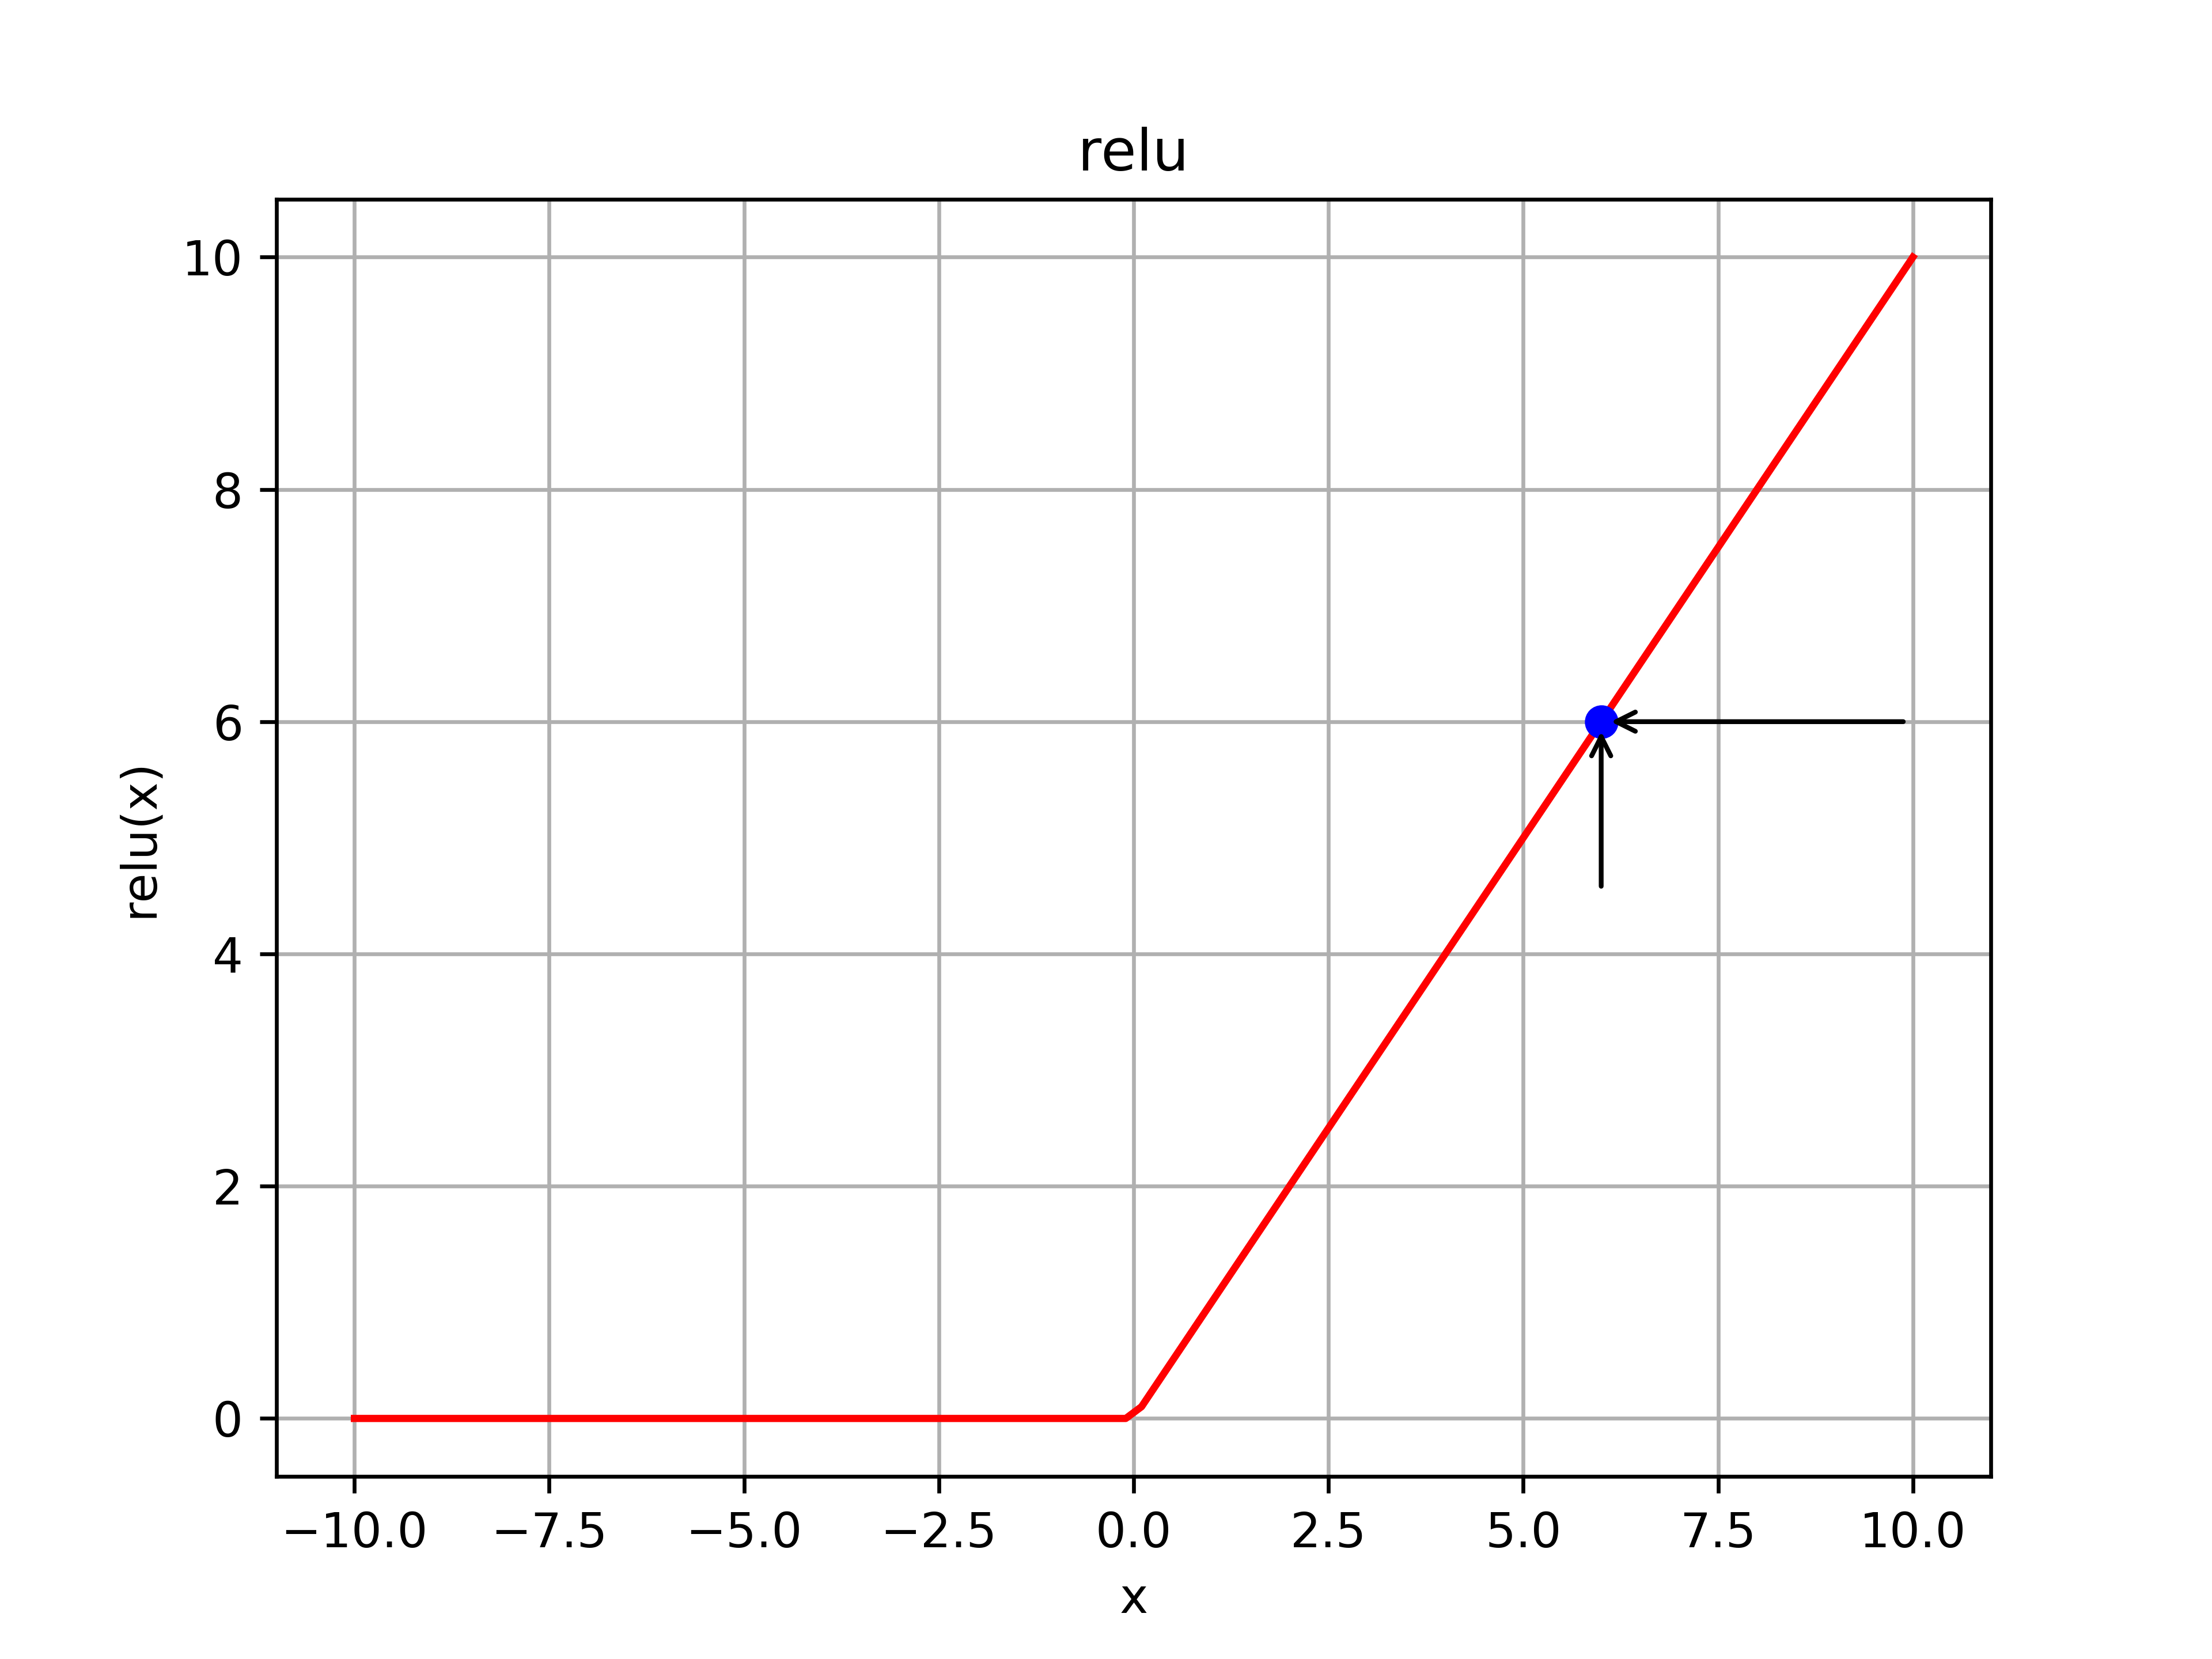
\includegraphics[scale=0.8]{./pic/chapter1/relu.png}
\caption{relu}
\end{figure}
\begin{figure}[H]
\centering
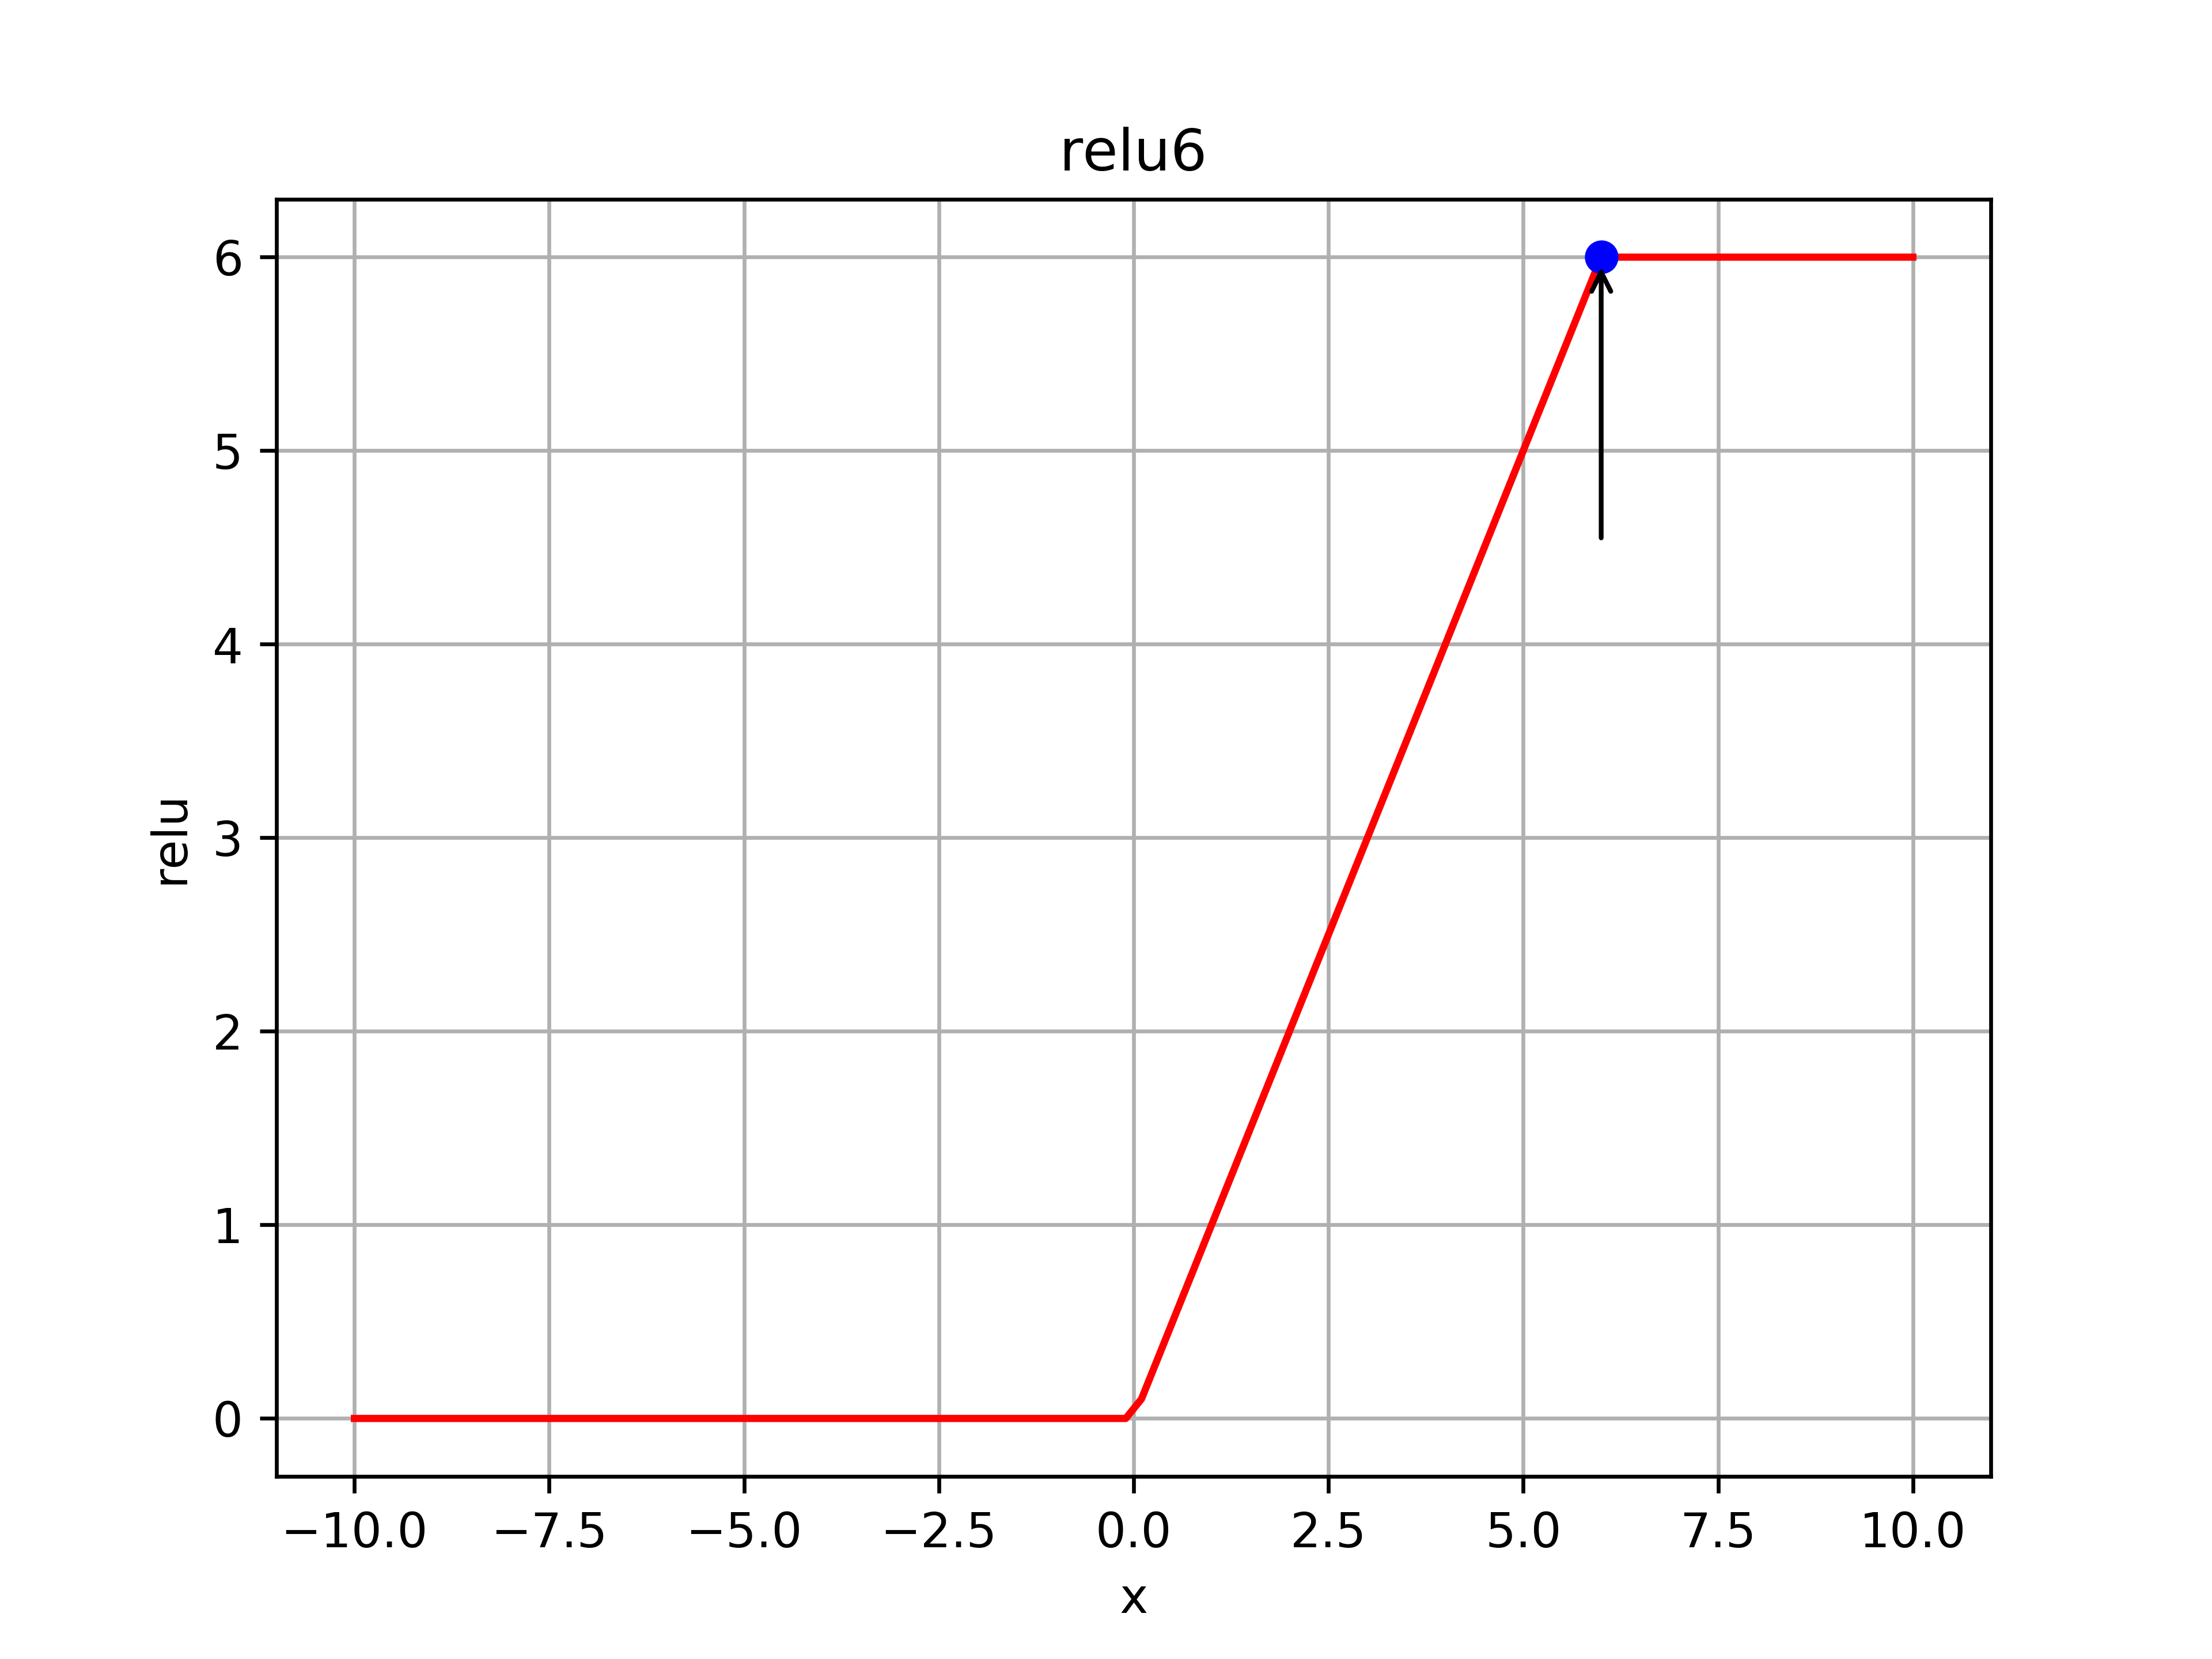
\includegraphics[scale=0.8]{./pic/chapter1/relu6.png}
\caption{relu6}
\end{figure}

\subsection{sigmoid}
\begin{python}
import tensorflow as tf 
import matplotlib.pyplot as plt 
import matplotlib.patches as mpatches
x = tf.linspace(-10.,10.,100)
y1 = tf.nn.sigmoid(x)
y2 = tf.nn.tanh(x)
red_patch = mpatches.Patch(color = 'red',label = 'sigmoid')
blue_patch = mpatches.Patch(color = 'blue',label = 'tanh')
with tf.Session() as sess:
	[x,y1,y2] = sess.run([x,y1,y2])
plt.plot(x,y1,'r',x,y2,'b')
ax = plt.gca()
ax.annotate(r"$tanh(x) = \frac{1-^{-2x}}{1+e^{-x}}$",
	   xy=(0,0),xycoords="data",
	   xytext=(1,0),textcoords="data",
	   arrowprops=dict(arrowstyle="->",
	   connectionstyle="arc3"),
)
ax.annotate(r"$sigmoid(x) = \frac{1}{1+e^{-x}}$",
	   xy=(0,0.5),xycoords="data",
	   xytext=(1,0.5),textcoords="data",
	   arrowprops=dict(arrowstyle="->",
	   connectionstyle="arc3"),
)
plt.xlabel('x')
plt.grid(True)
plt.legend(handles = [red\_patch,blue\_patch])
plt.savefig('activate.png',dpi=600)
\end{python}
\begin{figure}[H]
\centering
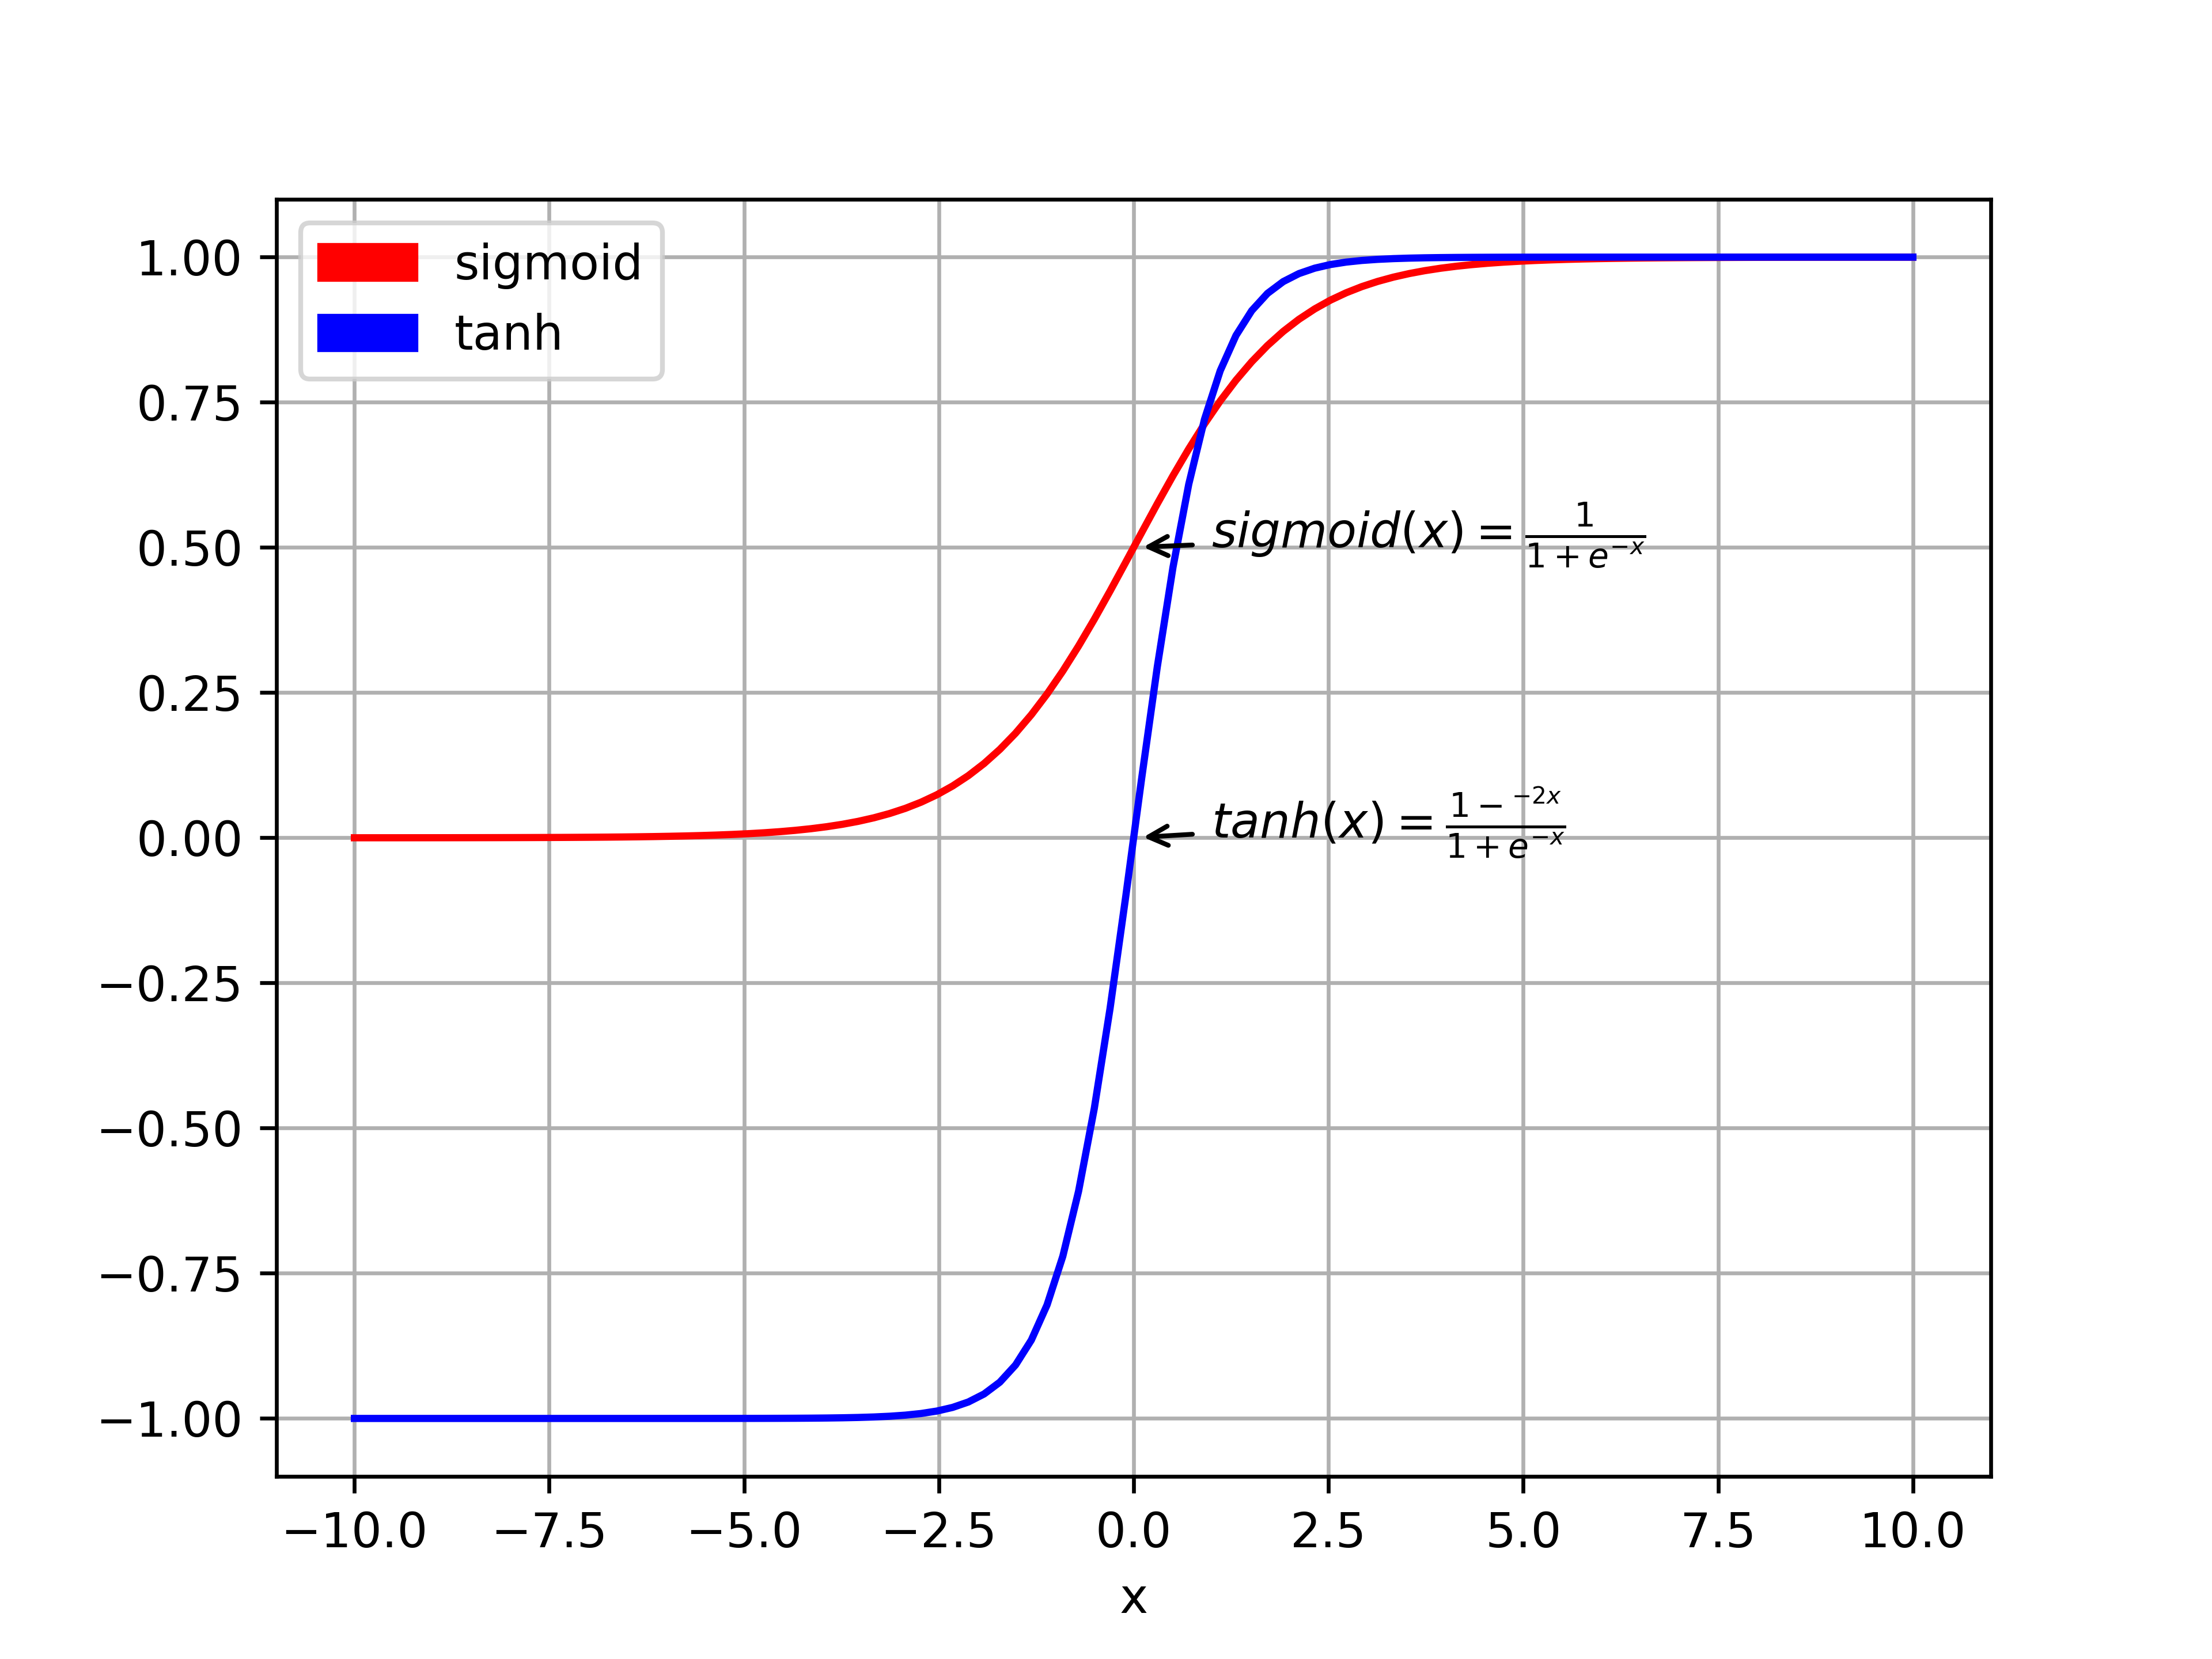
\includegraphics[scale=0.8]{./pic/chapter1/activate_fun.png}
\caption{activate\_fun}
\end{figure}
\subsection{relu和softplus}
\begin{python}
import tensorflow as tf 
import matplotlib.pyplot as plt 
import matplotlib.patches as mpatches
x = tf.linspace(-10.,10.,100)
y2 = tf.nn.softplus(x)
y3 = tf.nn.relu(x)
blue_patch = mpatches.Patch(color = 'blue',label = 'softplus')
yellow_patch = mpatches.Patch(color = 'yellow',label = 'relu')
with tf.Session() as sess:
	[x,y2,y3] = sess.run([x,y2,y3])
plt.plot(x,y2,'b',x,y3,'y')
ax = plt.gca()
plt.xlabel('x')
ax.annotate(r"$softplus(x)=log(1+e^x)$",
	   xy=(0,0),xycoords="data",
	   xytext=(1,0),textcoords="data",
	   arrowprops=dict(arrowstyle="->",
	   connectionstyle="arc3"),
)
ax.annotate(r"$relu(x)=max(x,0)$",
	   xy=(0,0.5),xycoords="data",
	   xytext=(1,0.5),textcoords="data",
	   arrowprops=dict(arrowstyle="->",
	   connectionstyle="arc3"),
)

plt.grid(True)
plt.legend(handles = [blue_patch,yellow_patch])
plt.savefig('relu_softplus.png',dpi=600)
\end{python}
\begin{figure}[H]
\centering
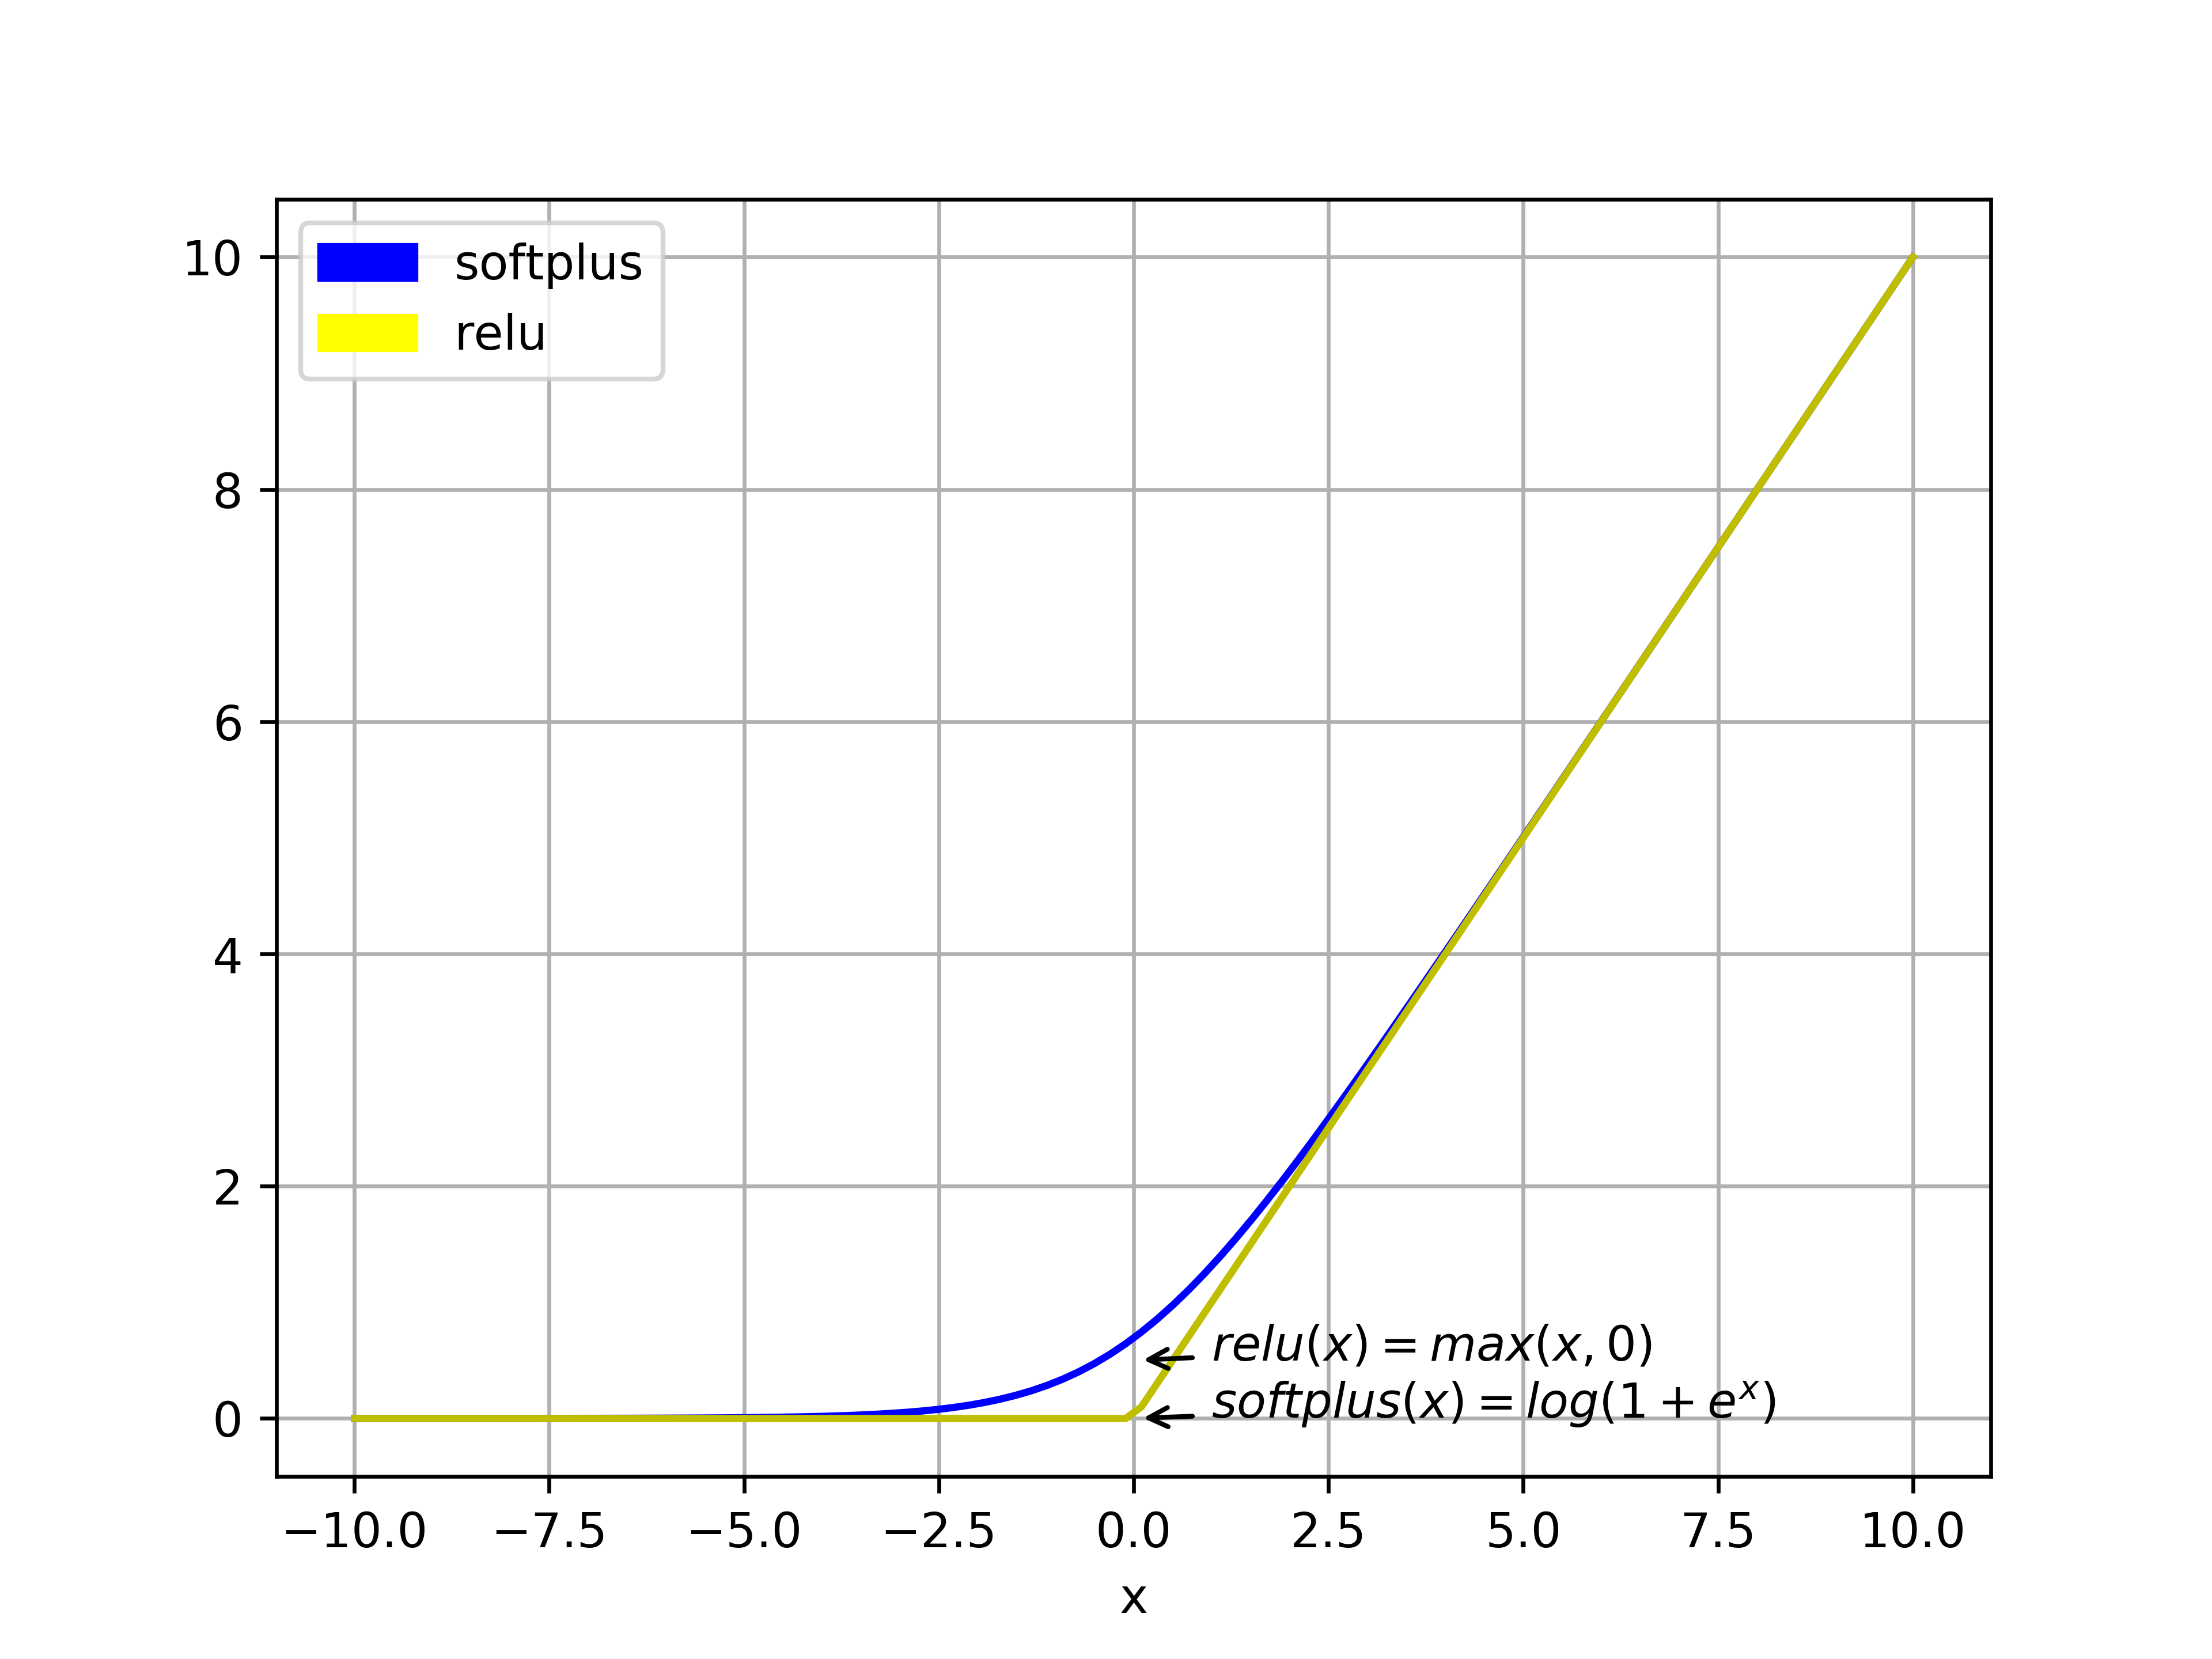
\includegraphics[scale=0.8]{./pic/chapter1/relu_softplus.png}
\end{figure}
\subsection{dropout}
将神经元以概率keep\_prob绝对是否被抑制。如果被抑制该神经元的输出为0如果不被抑制,该神经元的输出将被放大到原来的1/keep\_prop。
默认情况下,每个神经元是否被抑制是相互独立的。但是是否被抑制也可以通过noise\_shape来调节。当noise\_shape[i]=shape(x)[i]时,x中的元素相互独立。如果shape(x)=[k,1,1,n],那么每个批通道都是相互独立的,但是每行每列的数据都是关联的,也就是说要么都为0,要么还是原来的值。
\begin{python}
import tensorflow as tf
a = tf.constant([[-1.,2.,3.,4.]])
with tf.Session() as sess:
    b = tf.nn.dropout(a,0.5,noise_shape=[1,4])
    print(sess.run(b))
    c = tf.nn.dropout(a,0.5,noise_shape=[1,1])
    print(sess.run(c))
\end{python}
[[-2.  0.  0.  8.]]\newline
[[-0.  0.  0.  0.]]\newline
当输入数据特征相差明显时,用tanh效果会很好,但在循环过程中会不断扩大特征效果并显示出来。当特征相差不明显时,sigmoid效果比较好。同时,用sigmoid和tanh作为激活函数时,需要对输入进行规范化,否则激活厚的值全部进入平坦区,隐藏层的输出会趋同,丧失原来的特征表达,而relu会好很多,优势可以不需要输入规范化来避免上述情况。因此,现在大部分卷积神经网络都采用relu作为激活函数。
\section{CNN常用函数}
\subsection{卷积函数}
tf.nn.conv2d(input,filter,padding,stride=None,diation\_rate=Nonei每name = None,data\_format=None)\newline
\begin{itemize}
\item input:一个tensor,数据类型必须是float32,或者是float64
\item filter:一个tensor,数据类型必须和input相同。
\item strides:一个长度为4的一组证书类型数组,每一维对应input中每一维对应移动的步数,strides[1]对应input[1]移动的步数。
\item padding:有两个可选参数'VALID'(输入数据维度和输出数据维度不同)和'SAME'(输入数据维度和输出数据维度相同)
\item use\_cudnn\_on\_gpu:一个可选的布尔值,默认情况下时True。
\item name:可选,操作的一个名字。
\end{itemize}
\begin{python}
import tensorflow as tf
input_data = tf.Variable(tf.random_normal(shape = [10,9,9,3],mean=0,stddev=1),dtype = tf.float32)
kernel = tf.Variable(tf.random_normal(shape = [2,2,3,2],mean = 0,stddev=1,dtype=tf.float32))

y = tf.nn.conv2d(input_data,kernel,strides=[1,1,1,1],padding='SAME')
init = tf.global_variables_initializer()
with tf.Session() as sess:
    sess.run(init)
    print(sess.run(y).shape)
\end{python}
输出形状为[10,9,9,2]。
\subsection{池化}
\begin{tabular}{|p{15cm}|l|}
池化函数 &功能\\
\hline
\textcircled{1} tf.nn.avg\_pool(value,ksize,strides,padding,data\_format='NHWC',name =None)&平均池化\\
\textcircled{2} tf.nn.max\_pool(value,ksize,strides,padding,data\_format='NHWC',name =None)&最大池化\\
\textcircled{3} tf.nn.max\_pool\_with\_argmax(input,ksize,strides,padding,Targmax=None,name =None)&最大池化返回最大值的位置\\
\textcircled{4} tf.nn.avg\_pool3d(input,ksize,strides,padding,name =None)&三维状态下的平均池化\\
\textcircled{5} tf.nn.max\_pool3d(input,ksize,strides,padding,name =None)&三维状态下的最大池化\\
\textcircled{6} tf.nn.fractionan\_avg\_pool(value,pooling\_ratio,pseudo\_random=None,overlapping=None,deterministic=None,seed = None,seed2=None,name = None)&三维下的平均池化\\
\textcircled{7} tf.nn.avg\_max\_pool(value,pooling\_ratio,pseudo\_random=None,overlapping=None,deterministic=None,seed = None,seed2=None,name = None)&三维状态下的最大池化\\
\textcircled{8} tf.nn.pool(input,window\_shape,pool\_typing,padding,dilation\_rate = None,strides=None,name=None,data\_format=None)&执行一个N为池化操作。
\end{tabular}
\begin{itemize}
\item value:一个四维Tensor,维度时[batch,height,width,chennels]。
\item ksize:一个长度不小于4的整型数据,每一位上的值对应于输入数据Tensor中每一维窗口对应值。
\item stride:一个长度不小于4的整型列表。该参数指定窗口在输入数据Tensor每一维上的步长。
\item padding:一个字符串,取值为SAME或者VALID。
\item data\_format:NHWC。
\end{itemize}
\subsection{常见的分类函数}
tf.nn.sigmoid\_cross\_entropy\_with\_logits(logits,targets,name=None)
\begin{itemize}
	\item logits:[batch\_size,num\_classes]
	\item targets:[batch\_size,size]
	\item 输出:loss[batch\_size,num\_classes]
\end{itemize}
最后已成不需要进行sigmoid操作。\par
tf.nn.softmax(logits,dim=-1,name=None):计算Softmax
\[softmax = \frac{x^{logits}}{reduce\_sum(e^{logits},dim)}\]
tf.nn.log\_softmax(logits,dim=-1,name = None)计算log softmax
\[logsoftmax = logits-log(reduce\_softmax(exp(logits),dim))\]
tf.nn.softmax\_cross\_entropy\_with\_logits(\_setinel=None,labels=None,logits=None,dim=-1,name=None)
输出loss:[batch\_size]保存的时batch中每个样本的交叉熵。
tf.nn.sparse\_softmax\_cross\_entropy\_with\_logic(logits,labels,name=None)
\begin{itemize}
	\item logits:神经网络最后一层的结果。
	\item 输入logits:[batch\_size,num\_classes],labels:[batch\_size],必须在[0,num\_classes]
	\item loss[batch],保存的是batch每个样本的交叉熵。
\end{itemize}
\section{优化方法}
\begin{itemize}
	\item tf.train.GradientDescentOptimizer
	\item tf.train.AdadeltaOptimizer
	\item tf.train.AdagradDAOptimizer
	\item tf.train.AdagradOptimizer
	\item tf.train.MomentumOptimizer
	\item tf.train.AdamOptimizer
	\item tf.train.FtrlOptimizer
	\item tf.train.RMSPropOptimizer
\end{itemize}
\subsection{BGD}
BGD(batch gradient descent)批量梯度下降。这种方法是利用现有的参数对训练集中的每一个输入生成一个估计输出$y_i$,然后跟实际的输出$y_i$比较,统计所有的误差,求平均后的到平均误差作为更新参数的依据。啊他的迭代过程是:
\begin{enumerate}
	\item 提取巡检集中所有内容$\{x_1,\ldots,x_n\}$,以及相关的输出$y_i$;
	\item 计算梯度和误差并更新参数。
\end{enumerate}
这种方法的优点是:使用所有数据计算,都保证收敛,并且并不需要减少学习率缺点是每一步需要使用所有的训练数据,随着训练的进行,速度会变慢。那么如果将训练数据拆分成一个个batch,每次抽取一个batch数据更新参数,是不是能加速训练?这就是SGD。
\subsection{SGD}
SGD(stochastic gradient descent):随机梯度下降。这种方法的主要思想是将数据集才分成一个个的batch,随机抽取一个batch计算并更新参数,所以也称为MBGD(minibatch gradient descent)\
SGD在每次迭代计算mini-batch的梯度,然后队参数进行更新。和BGD相比,SGD在训练数据集很大时也能以较快的速度收敛,但是它有两个缺点:
\begin{enumerate}
\item 需要手动调整学习率,但是选择合适的学习率比较困难。尤其在训练时,我们常常想队常出现的特征更新速度快点,队不长出现的特征更新速度慢些,而SGD对更新参数时对所有参数采用一样的学习率,因此无法满足要求。
\item SGD:容易收敛到局部最优。
\end{enumerate}
\subsection{momentum}
Momentum时模拟物理学中的动量概念,更新时在一定程度上保留之前的更新方向,利用当前批次再次微调本次更新参数,因此引入了一个新的变量v,作为前几次梯度的累加。因此,momentum能够更新学习率,在下降初期,前后梯度方向一致时能加速学习:在下降的中后期,在局部最小值附近来回振荡,能够抑制振荡加快收敛。
\subsection{Nesterov Momentum}
标准的Monentum法首先计算一个梯度,然后子啊加速更新梯度的方向进行一个大的跳跃Nesterov首先在原来加速的梯度方向进行一个大的跳跃,然后在改为值设置计算梯度值,然后用这个梯度值修正最终的更新方向。
\subsection{Adagrad}
Adagrade能够自适应的为哥哥参数分配不同的学习率,能够控制每个维度的梯度方向,这种方法的优点是能实现学习率的自动更改,如果本次更新时梯度大,学习率就衰减得快,如果这次更新时梯度小,学习率衰减得就慢些。
\subsection{RMSprop}
和Momentum类似,通过引入衰减系数使得每个回合都衰减一定比例。在实践中,对循环神经网络效果很好。
\subsection{Adam}
名称来自自适应矩阵(adaptive moment estimation).Adam更均损失函数针对每个参数的一阶矩,二阶矩估计动态调整每个参数的学习率。
\begin{python}
import numpy as np
import tensorflow as tf
import matplotlib.pyplot as plt
tf.set_random_seed(0)
np.random.seed(0)
LR = 0.01
BATCH_SIZE = 32
x = np.linspace(-1,1,100).reshape(-1,1)
noise = np.random.normal(0,0.1,size=x.shape)
y = np.power(x,2)+noise
class Net:
    def __init__(self,opt,**kwargs):
        self.x = tf.placeholder(tf.float32,[None,1])
        self.y = tf.placeholder(tf.float32,[None,1])
        l = tf.layers.dense(self.x,20,tf.nn.relu)
        out = tf.layers.dense(l,1)
        self.loss = tf.losses.mean_squared_error(self.y,out)
        self.train = opt(LR,**kwargs).minimize(self.loss)
net_SGD = Net(tf.train.GradientDescentOptimizer)
net_momentum = Net(tf.train.MomentumOptimizer,momentum=0.9)
net_RMSprop = Net(tf.train.RMSPropOptimizer)
net_Adam = Net(tf.train.AdamOptimizer)
nets = [net_SGD,net_momentum,net_RMSprop,net_Adam]
sess = tf.Session()
sess.run(tf.global_variables_initializer())
losses_his = [[],[],[]]
for step in range(300):
    index = np.random.randint(0,x.shape[0],BATCH_SIZE)
    b_x = x[index]
    b_y = y[index]
    for net,l_his in zip(nets,losses_his):
        _,l = sess.run([net.train,net.loss],{net.x:b_x,net.y:b_y})
        l_his.append(l)
labels = ['SGD','Momentum','RMSprop','Adam']
for i,l_his in enumerate(losses_his):
    plt.plot(l_his,label=labels[i])
plt.legend(loc='best')
plt.xlabel('Step')
plt.ylabel('Loss')
plt.ylim(0,0.2)
plt.savefig('Opt.png',dpi=600)
\end{python}
\begin{figure}[H]
	\centering
	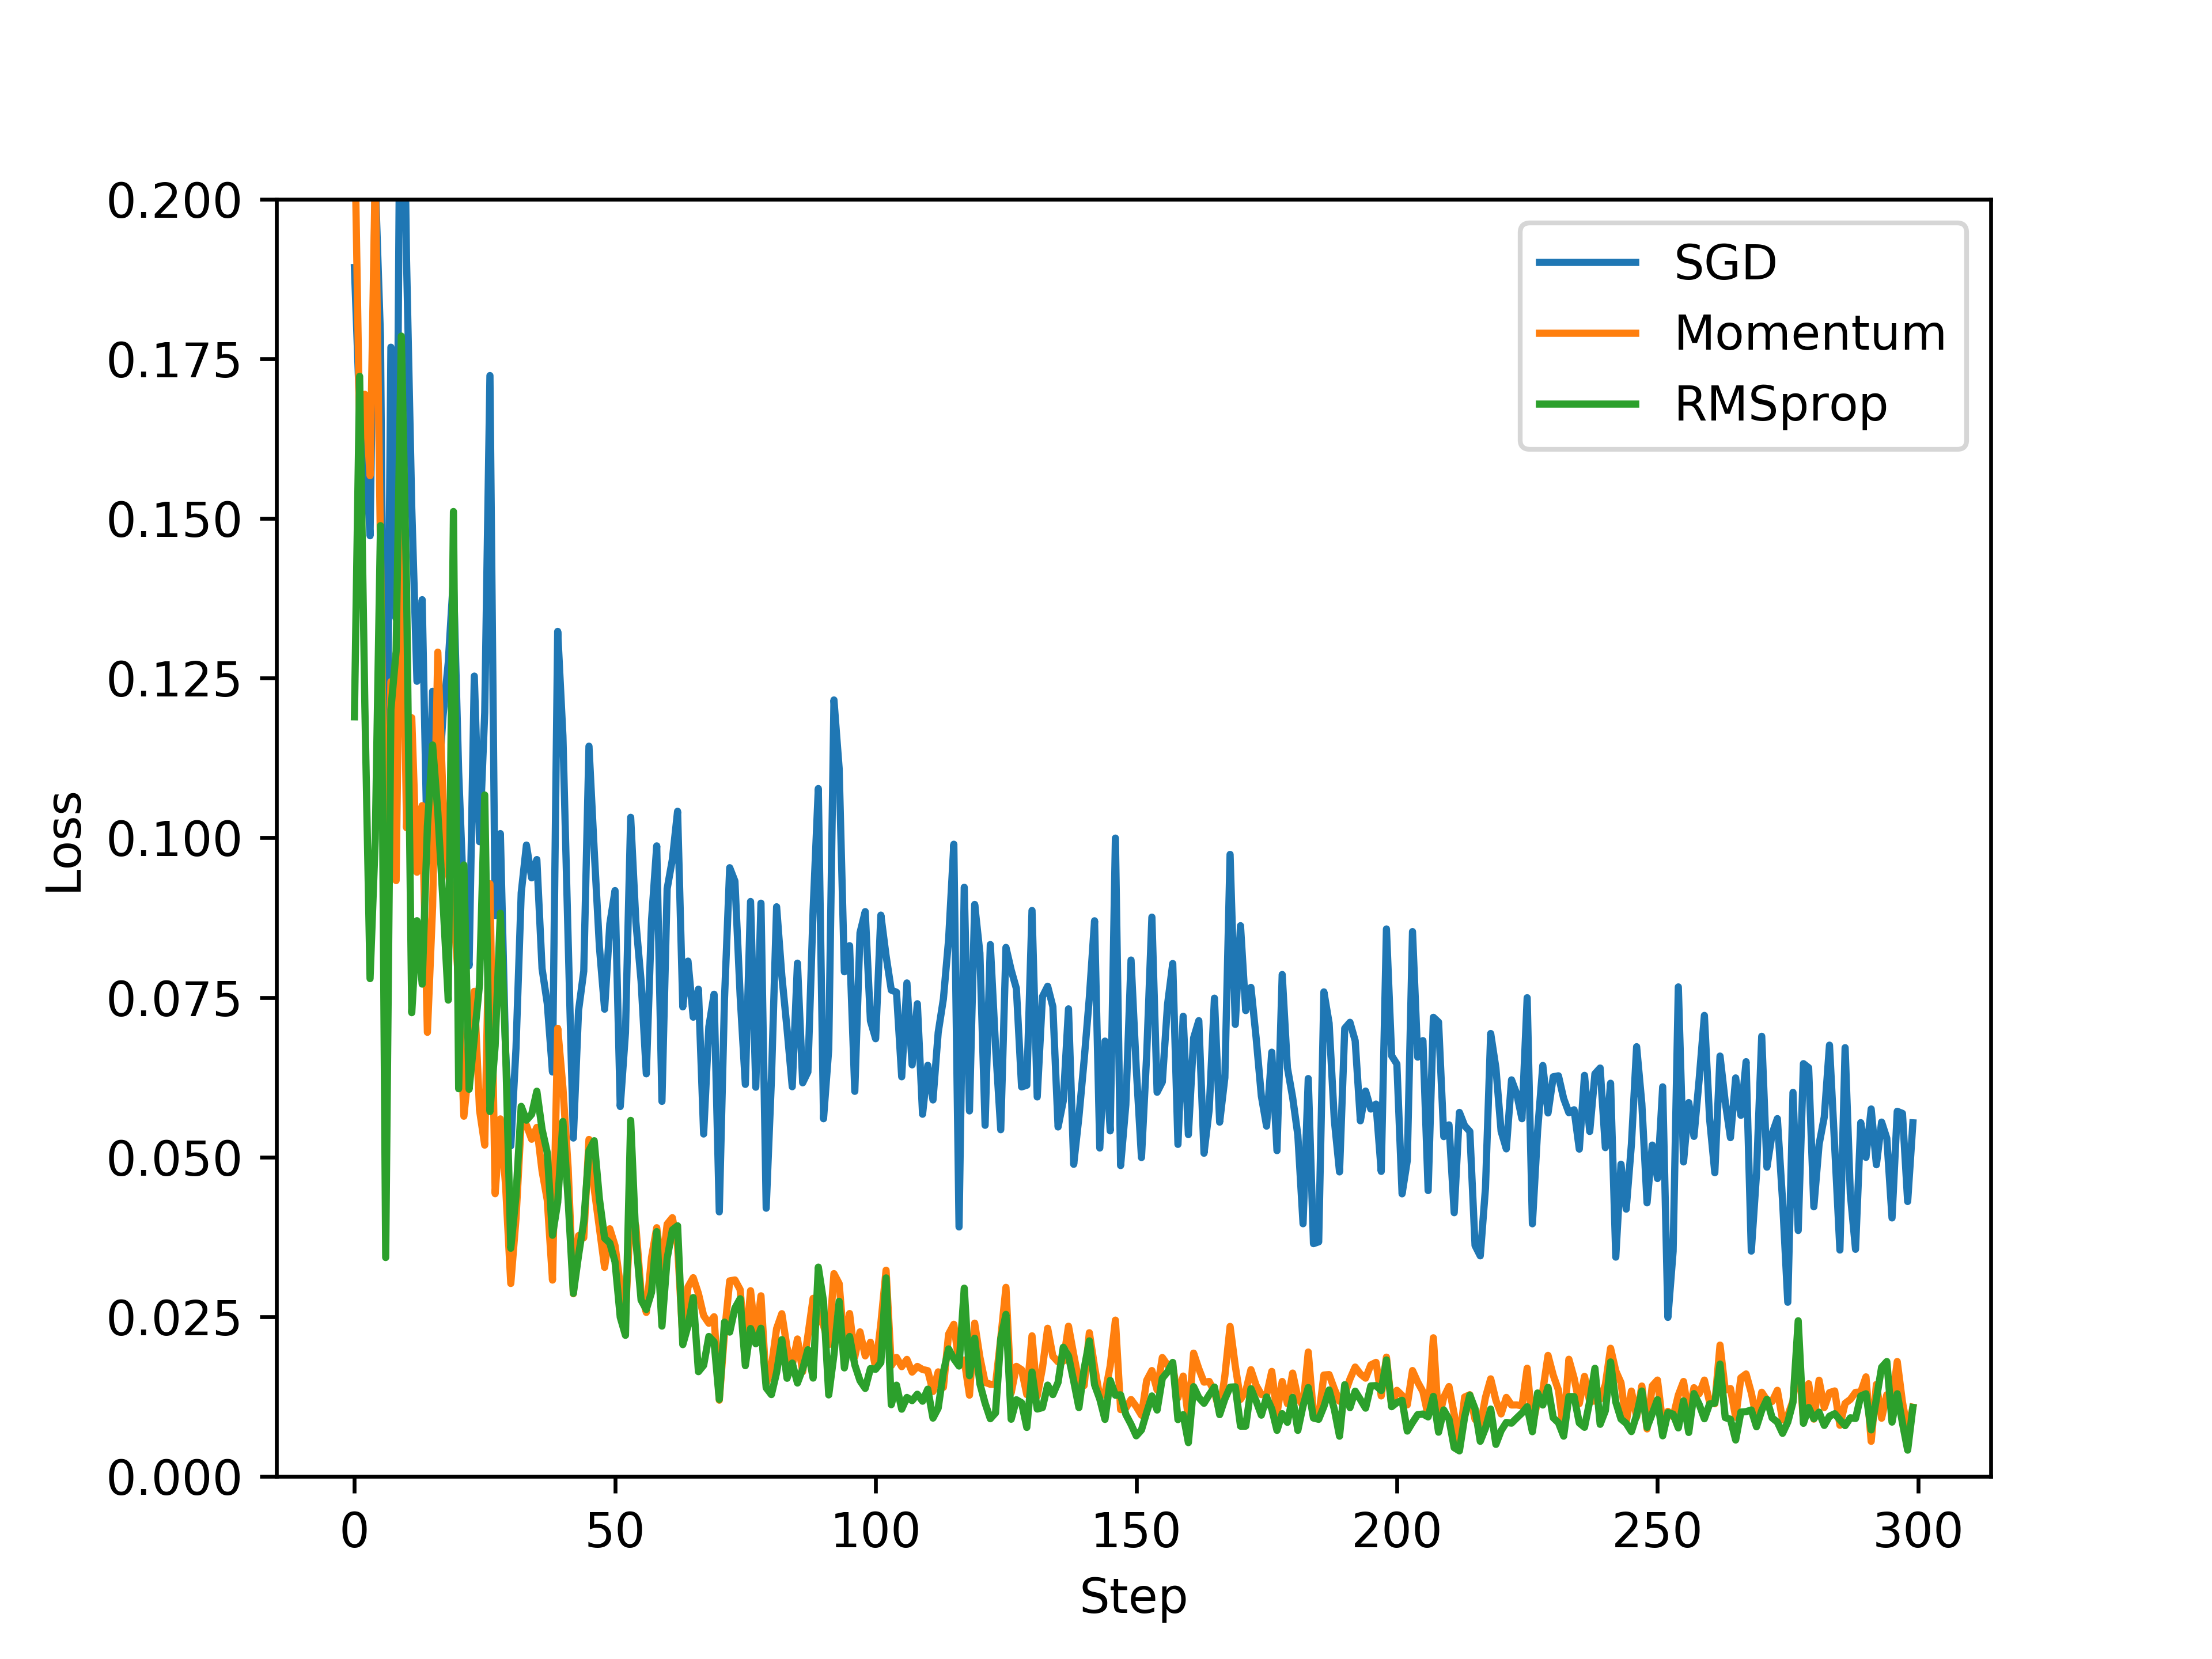
\includegraphics[scale=0.6]{./pic/chapter1/Opt.png}
\end{figure}
\subsection{构造简单的神经网络拟合数据}
原始数据为$y=x^2$的基础上添加随机噪声。原始数据的散点图如下
\begin{center}
\begin{figure}[H]
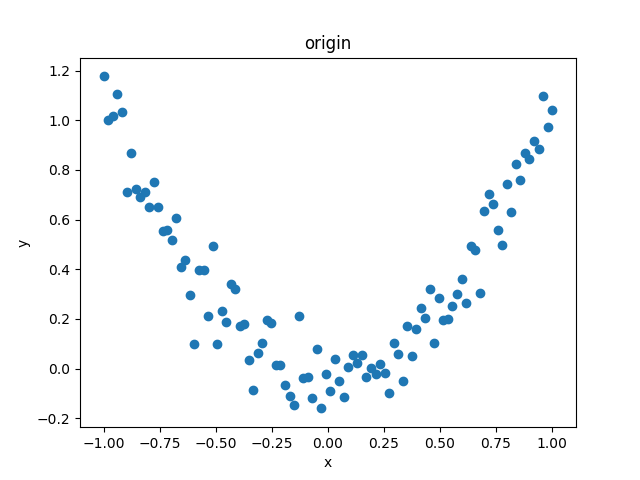
\includegraphics[scale=0.6]{./pic/chapter1/origin.png}
\end{figure}
\end{center}
\begin{python}
#tensorflow 1.2.1
import tensorflow as tf
import matplotlib.pyplot as plt
import numpy as np
tf.set_random_seed(0)
np.random.seed(0)
#生成数据
step = 100
x = np.linspace(-1,1,step).reshape(-1,1)
noise = np.random.normal(0,0.1,size=x.shape)
y = np.power(x,2)+noise

tf_x = tf.placeholder(tf.float32,x.shape)
tf_y = tf.placeholder(tf.float32,x.shape)
l1 =  tf.layers.dense(tf_x,10,tf.nn.relu)
output = tf.layers.dense(l1,1)

loss = tf.losses.mean_squared_error(tf_y,output)
optimizer = tf.train.GradientDescentOptimizer(learning_rate=0.5)
train_op = optimizer.minimize(loss)

sess = tf.Session()
sess.run(tf.global_variables_initializer())
plt.ion()
for step in range(100):
    _,l,pred = sess.run([train_op,loss,output],{tf_x:x,tf_y:y})
    if step%5==0:
        plt.cla()
        plt.scatter(x,y)
        plt.title(r'$y=x^2+noise$')
        plt.plot(x,pred,'r-',lw=2)
        plt.text(0,0.8,'Loss=%.4f'%l,fontdict={'size':10,'color':'blue'})
        plt.xlabel("x")
        plt.ylabel(r"$y=x^2$")
        plt.pause(0.1)
plt.ioff()
plt.show()
\end{python}
最终拟合数据:
\begin{figure}[H]
\includegraphics[scale=0.4]{./pic/chapter1/final.png}
\end{figure}
\section{TensorBoard}
\begin{python}
import tensorflow as tf
import matplotlib.pyplot as plt

tf.set_random_seed(1)
x0 = tf.random_normal((100,2),2,2,tf.float32,0)
y0 = tf.zeros(100)
x1 = tf.random_normal((100,2),-2,2,tf.float32,0)
y1 = tf.ones(100)
x = tf.reshape(tf.stack((x0,x1),axis=1),(200,2))
y = tf.reshape(tf.stack((y0,y1),axis=1),(200,1))
with tf.Session() as sess:
    x = sess.run(x)
    y = sess.run(y)

tf_x = tf.placeholder(tf.float32, x.shape)     # input x
tf_y = tf.placeholder(tf.int32, y.shape)     # input y

# neural network layers
l1 = tf.layers.dense(tf_x, 10, tf.nn.relu)          # hidden layer
output = tf.layers.dense(l1, 2)                     # output layer

loss = tf.losses.sparse_softmax_cross_entropy(labels=tf_y, logits=output)           # compute cost
accuracy = tf.metrics.accuracy(          # return (acc, update_op), and create 2 local variables
            labels=tf.squeeze(tf_y), predictions=tf.argmax(output, axis=1),)[1]
optimizer = tf.train.GradientDescentOptimizer(learning_rate=0.05)
train_op = optimizer.minimize(loss)

sess = tf.Session()                                                                 # control training and others
init_op = tf.group(tf.global_variables_initializer(), tf.local_variables_initializer())
sess.run(init_op)     # initialize var in graph

plt.ion()   # something about plotting
for step in range(100):
    _, acc, pred = sess.run([train_op, accuracy, output], {tf_x: x, tf_y: y})
    if step % 2 == 0:
        plt.cla()
        plt.scatter(x[:, 0], x[:, 1], c=pred.argmax(1), s=100, lw=0, cmap='RdYlGn')
        plt.text(1.5, -4, 'Accuracy=%.2f' % acc, fontdict={'size': 20, 'color': 'red'})
        plt.pause(0.1)
plt.ioff()
plt.show()
\end{python}
\begin{figure}[H]
	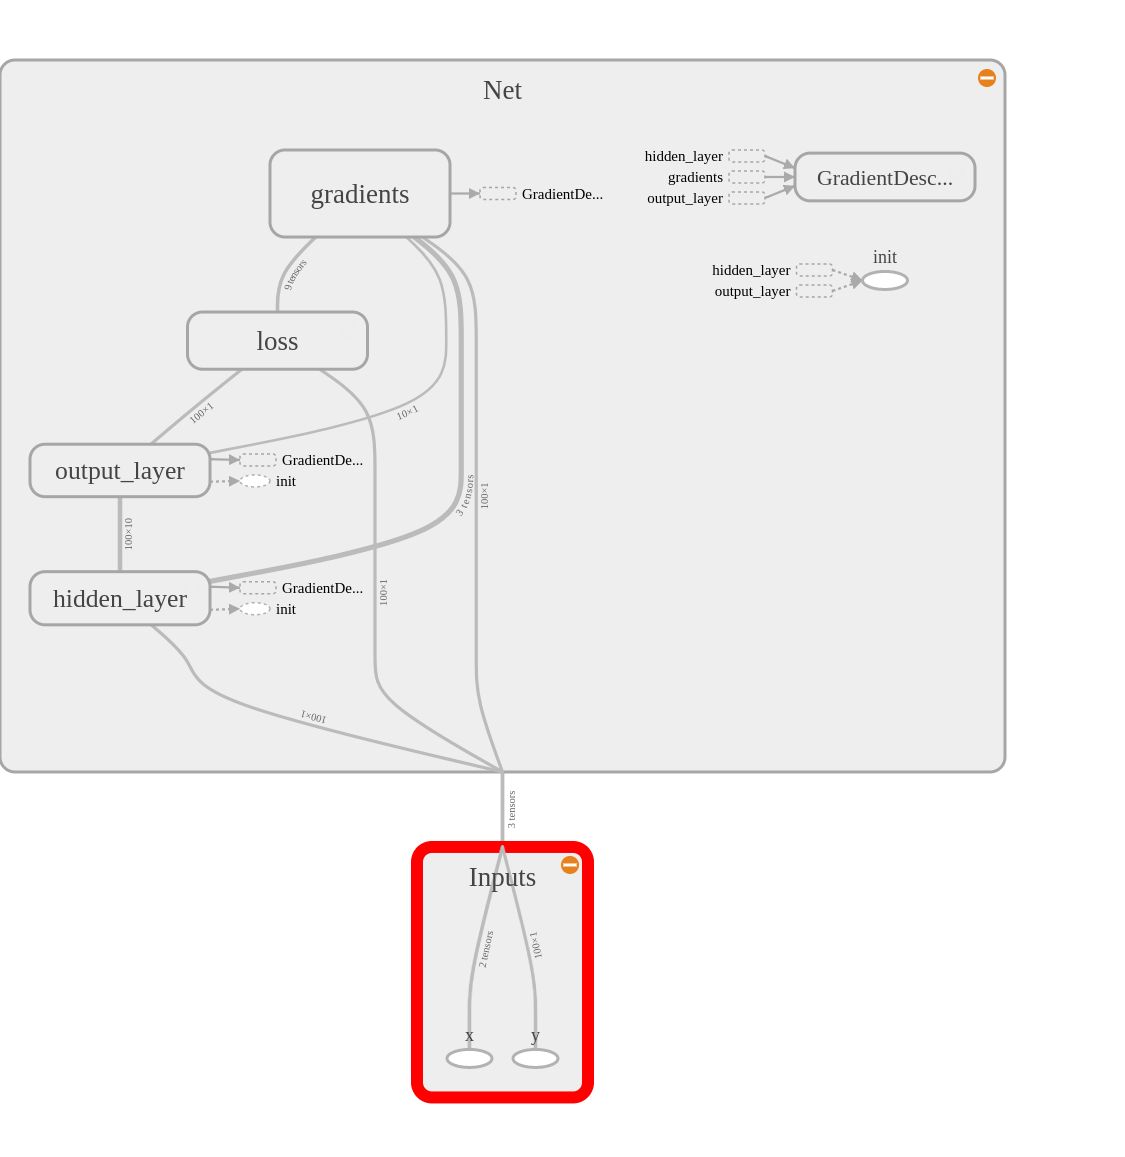
\includegraphics[scale=0.4]{./pic/chapter1/tenbor1.png}
\end{figure}
\subsection{TensorBoard Histogram Dashboard}
TensorBoard Histogram Dashboard 显示TensorFlow图中的Tensor如何随着时间变化。
\subsection{自编码}
人工神经网络(ANN)本身就是具有层次结构的系统,如果给定一个神经网络,我们假设其输出与输入是相同的,然后训练调整其参数,得到每一层中的权重。自然地,我们就得到了输入I的几种不同表示(每一层代表一种表示),这些表示就是特征。在研究中可以发现,如果在原有的特征中加入这些自动学习得到的特征可以大大提高精确度,甚至在分类问题中比目前最好的分类算法效果还要好!这种方法称为AutoEncoder(自动编码器)。自动编码器就是一种尽可能复现输入信号的神经网络。为了实现这种复现,自动编码器就必须捕捉可以代表输入数据的最重要的因素,就像PCA那样,找到可以代表原信息的主要成分。
我们将input输入一个encoder编码器,就会得到一个code,这个code也就是输入的一个表示,那么我们怎么知道这个code表示的就是input呢?我们加一个decoder解码器,这时候decoder就会输出一个信息,那么如果输出的这个信息和一开始的输入信号input是很像的(理想情况下就是一样的),那很明显,我们就有理由相信这个code是靠谱的。所以,我们就通过调整encoder和decoder的参数,使得重构误差最小,这时候我们就得到了输入input信号的第一个表示了,也就是编码code了。因为是无标签数据,所以误差的来源就是直接重构后与原输入相比得到。
\subsection{手写体数据自编码}
\begin{python}
import tensorflow as tf
#import numpy as np
import matplotlib.pyplot as plt
data_path = '/home/hpc/文档/mnist_tutorial/mnist'
from tensorflow.examples.tutorials.mnist import input_data
mnist = input_data.read_data_sets(data_path, one_hot=False)


# Visualize decoder setting
learning_rate = 0.01
training_epochs = 5
batch_size = 256
display_step = 1
examples_to_show = 10

n_input = 784  # MNIST data input (img shape: 28*28)

x = tf.placeholder(tf.float32,[None,n_input])

n_hidden_1 = 256
n_hidden_2 = 128
weights = {'encode_h1':tf.Variable(tf.random_normal([n_input,n_hidden_1])),
    'encode_h2':tf.Variable(tf.random_normal([n_hidden_1,n_hidden_2])),
    'decode_h2':tf.Variable(tf.random_normal([n_hidden_2,n_hidden_1])),
    'decode_h1':tf.Variable(tf.random_normal([n_hidden_1,n_input]))

}
bias = {'encode_h1':tf.Variable(tf.random_normal([n_hidden_1])),
    'encode_h2':tf.Variable(tf.random_normal([n_hidden_2])),
    'decode_h2':tf.Variable(tf.random_normal([n_hidden_1])),
    'decode_h1':tf.Variable(tf.random_normal([n_input]))

}
def encode(x):
    layer_1 = tf.nn.sigmoid(tf.add(tf.matmul(x,weights['encode_h1']),bias['encode_h1']))
    layer_2 = tf.nn.sigmoid(tf.add(tf.matmul(layer_1,weights['encode_h2']),bias['encode_h2']))
    return layer_2

def decode(x):
    layer_1 = tf.add(tf.matmul(x,weights['decode_h2']),bias['decode_h2'])
    layer_2 = tf.add(tf.matmul(layer_1,weights['decode_h1']),bias['decode_h1'])
    return layer_2



encode_op = encode(x)
decode_op = decode(encode_op)
y_pred = decode_op
y_true = x
cost = tf.reduce_mean(tf.square(y_pred-y_true))
optimizer = tf.train.AdamOptimizer(learning_rate).minimize(cost)

with tf.Session() as sess:
    init = tf.global_variables_initializer()
    sess.run(init)
    total_batch = int(mnist.train.num_examples/batch_size)
    for epoch in range(training_epochs):
        for i in range(total_batch):
            batch_xs,batch_ys = mnist.train.next_batch(batch_size)
#            _,c = sess.run([optimizer,cost],feed_dict={x:batch_xs})
            _, c = sess.run([optimizer, cost], feed_dict={x: batch_xs})
        if epoch%display_step==0:
            print("Epoch:",'%04d'%(epoch+1),'cost=','{:.9f}'.format(c))
    print('Optimize finish')
    encode_decode = sess.run(y_pred,feed_dict={x:mnist.test.images[:examples_to_show]})
    f,a = plt.subplots(2,10,figsize=(10,2))
    for i in range(examples_to_show):
        a[0][i].imshow(sess.run(tf.reshape(mnist.test.images[i],[28,28])))
        a[1][i].imshow(sess.run(tf.reshape(encode_decode[i],[28,28])))
    plt.show()
\end{python}
\begin{center}
\begin{figure}[H]
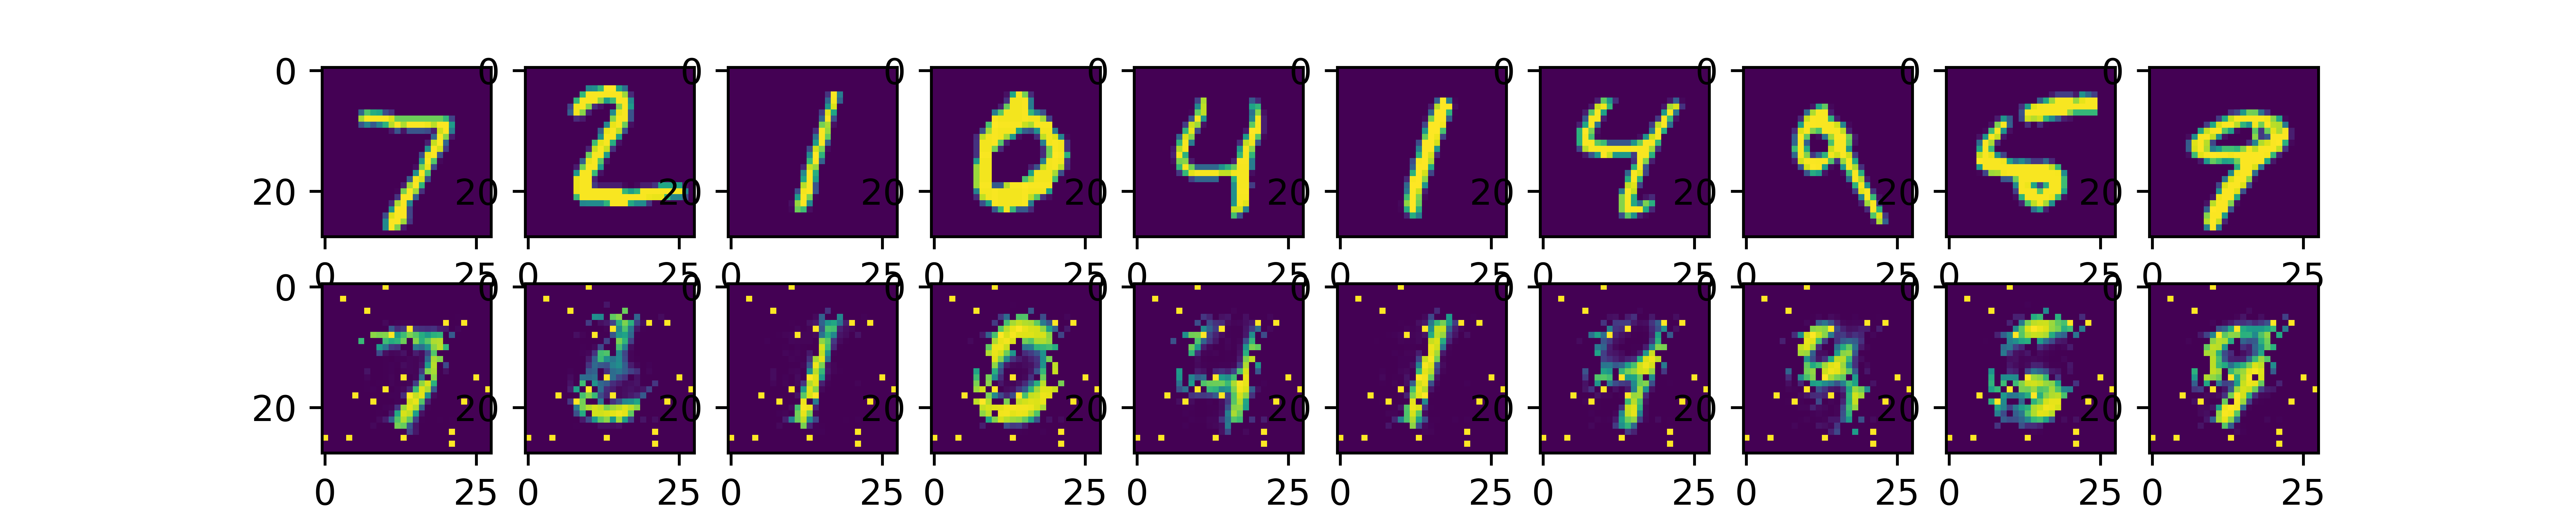
\includegraphics[scale=0.5]{auto_encode.png}
\end{figure}
\end{center}
\subsection{一个简单的例子}
正态分布变量,均值随着和时间移动。TensorFlow有一个操作tf.random\_normal可以完美的达到这个目的。正如通常情况下TensorBoard,我们将用summary op融合数据据。
在这种情况下'tf.summary.histogram'。
这里有一个代码段将生成一些包含正态分布直方图数据的总结,这里均值随着时间增大。
\begin{python}
import tensorflow as tf
k = tf.placeholder(tf.float32)
mean_moving_normal = tf.random_normal(shape=[1000], mean=(5*k), stddev=1)
summaries = tf.summary.histogram('normal/moving_mean',mean_moving_normal)
sess = tf.Session()
writer = tf.summary.FileWriter('./histogram_example')
N = 400
for step in range(N):
    k_val = step/float(N)
    summ = sess.run(summaries,feed_dict={k:k_val})
    writer.add_summary(summ,global_step=step)
\end{python}
在当前代码中运行下边的代码启动TensorFlow载入数据
\begin{python}
tensorboard --logdir=./histogram_example
\end{python}
\begin{center}
\begin{figure}[H]
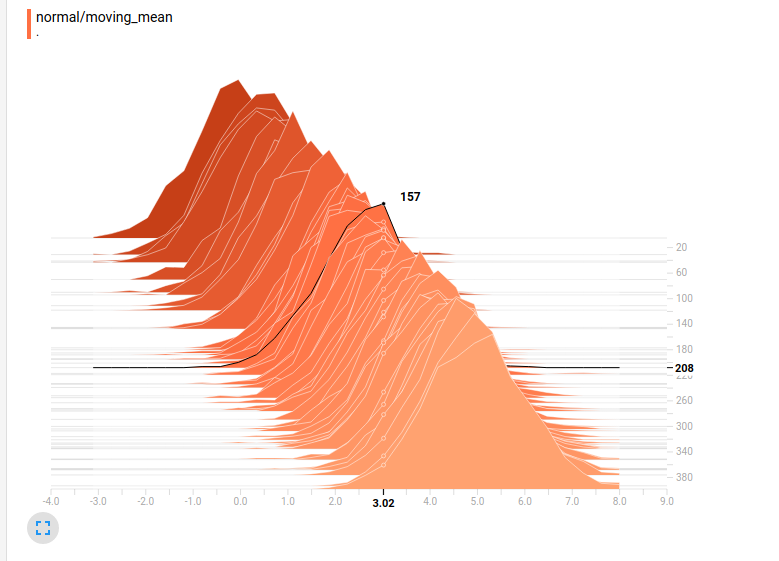
\includegraphics[scale=0.5]{tb_hist1.png}
\end{figure}
\end{center}
tf.summary.histogram接受任一尺寸和大小的Tensor,压缩他们进入直方数据结构组成一些小的数据宽度和数量组层的bin将诶够,例如我们像组成数[0.5,1.1,1.3,2.2,2.9,2.99]成3个bin,我们可以创建三个bin:一个包含0到1之间的一切(0.5),一个包含1-2(1.1,1.3)之间,一个包含2-3(2.2,2.9,2.99)

  TensorFlow用类是的方法创建bins,但是不想我们上面的例子,它不创建整数读额bins,瑞与大型数据,稀疏数据,这样的也许导致上千个bin,bins时指数分布时,一些bins相比于一些非常大数的bin接近于0。然而,可视化指数分布bin时一个技巧,如果高被编码为数量,bin宽度更大的空间,甚至他们有相同的元素,相比较之下统计数量使得豪赌比较变得可能,直方图采集数据仅均匀的bins,这可能导致不幸的人工操作。

在直方图可视化器的每一个切片显示为一个单个的直方图。切片安装步数组织。例老的切片(e.g. step 0)比较靠后变为更深,然而新的slices接近于前景色,颜色更轻,右边的y轴显示了步数。

你可以在直方图上滑动鼠标看到更多的详细星系。你如下面的图你可以看到直方图的时间不为177有一个bin中心在3.78有bin中有34.5个元素。
\begin{center}
\begin{figure}[H]
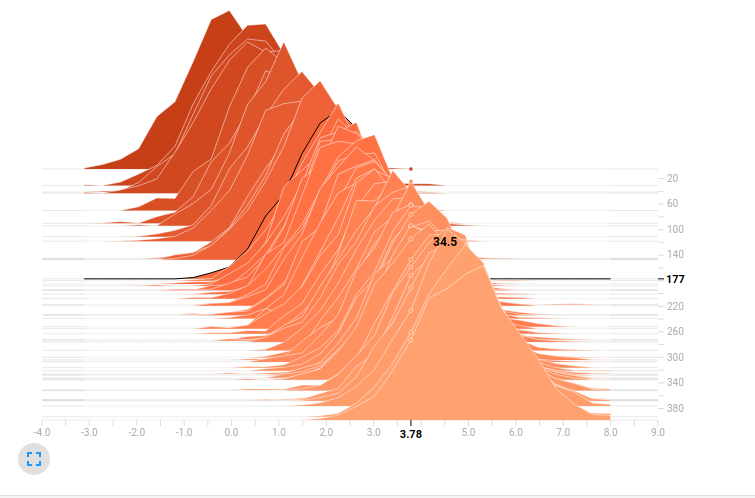
\includegraphics[scale=0.5]{tb_hist2.png}
\end{figure}
\end{center}
你也许注意到注意到直方切片在统计步数和时间上不总是偶数,这是因为TensorBoard用\href{https://en.wikipedia.org/wiki/Reservoir\_sampling}{reservoir sampling}保持直方图的子集,为了节约内存,Reservior sampling保证每个采样有一个相等的可能性被包含进去,但是因为它时一个随机算法,采样并不在每个偶数步发生。
\subsection{Overlay Mode}
控制面板上允许你打开直方图模式为offset为overlay。
在offset模式下,可视化转动45度,因此单个的直方图切片不再展开,而是所有的图华仔一个相同的y轴上。
\begin{center}
\begin{figure}[H]
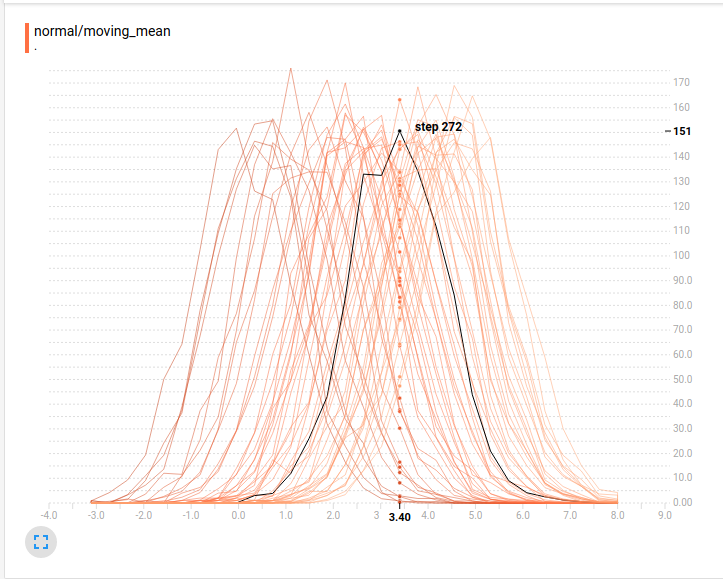
\includegraphics[scale=0.5]{tb_hist3.png}
\end{figure}
\end{center}
现在表上的每个切片被线分开,y轴显示每个bucket项目数量,深色线时老的,早期的时间不,浅色线时最近的新的时间不,你可以用鼠标在表上查看更多的信息。
\begin{center}
\begin{figure}[H]
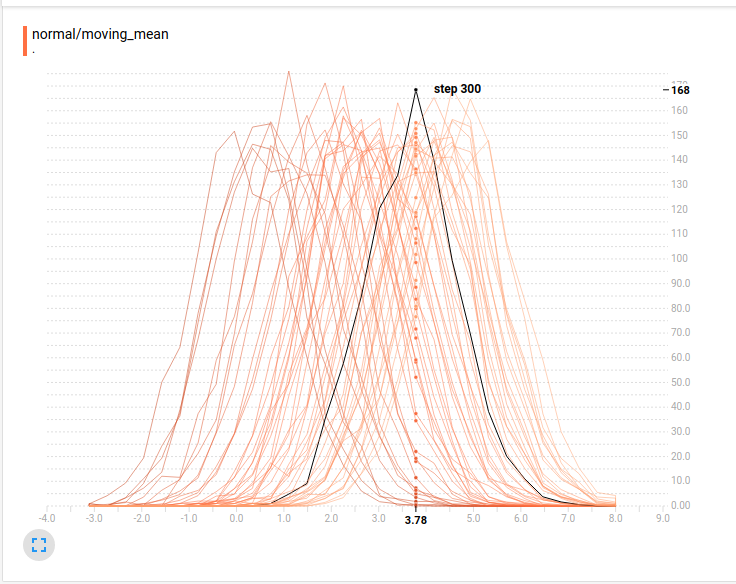
\includegraphics[scale=0.5]{tb_hist4.png}
\end{figure}
\end{center}

overlay可视化在你想直接比较不同直方图的数量。
\subsection{多个分布}
直方图控制面板对多分布下的可视化很有用,当我们通过链接两个不同的正态分布构造一个简单的二两分布,代码如下:
\begin{python}
import tensorflow as tf
k = tf.placeholder(tf.float32)
mean_moving_normal = tf.random_normal(shape=[1000],mean=(3*5),stddev=1)
tf.summary.histogram('normal/moving_mean',mean_moving_normal)
variance_shrinking_normal = tf.random_normal(shape=[100],mean=0,stddev=1-(k))
tf.summary.histogram('normal/shrinking_varance',variance_shrinking_normal)
normal_combined = tf.concat([mean_moving_normal,variance_shrinking_normal],0)
tf.summary.histogram('normal/bimodal',normal_combined)
summaris = tf.summary.merge_all()
sess = tf.Session()
writer = tf.summary.FileWriter('./histgram_example1')
N = 400
for step in range(N):
    k_val = step/float(N)
    summ = sess.run(summaris,feed_dict={k:k_val})
    writer.add_summary(summ,global_step=step)
\end{python}
上面的例子是滑动平均,现在我们已有一个收缩的变量分布。
\begin{center}
\begin{figure}[H]
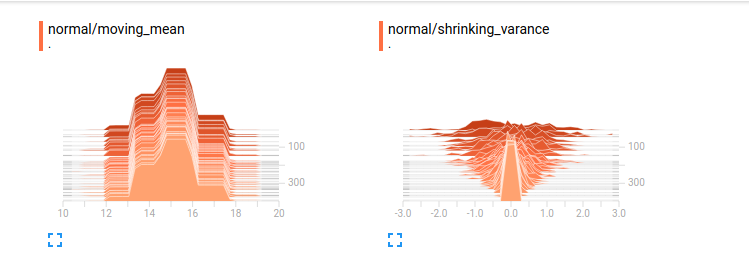
\includegraphics[scale=0.6]{tb_hist5.png}
\end{figure}
\end{center}
当我们链接她们在一起,我们得到一个清晰解释分歧,二进制结构的表格:
\begin{center}
\begin{figure}[H]
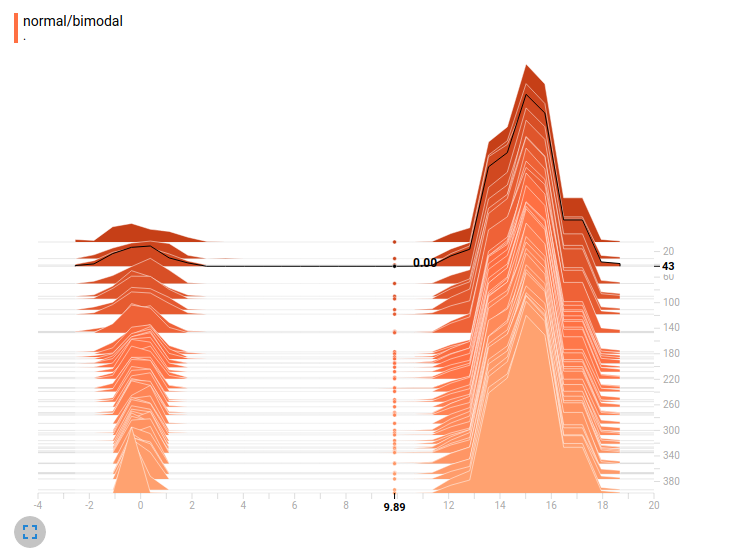
\includegraphics[scale=0.5]{tb_hist6.png}
\end{figure}
\end{center}
\subsection{更多分布}
生成可视化更多分布,结合他们到表中:
\begin{python}
import tensorflow as tf
k = tf.placeholder(tf.float32)
# Make a normal distribution,with a shift mean
mean_moving_normal = tf.random_normal(shape=[1000],mean=(5*k),stddev=1)
tf.summary.histogram('normal/moving_mean',mean_moving_normal)
variance_shrinking_normal = tf.random_normal(shape=[1000],mean=0,stddev=1-(k))
tf.summary.histogram('normal/shinking_variance',variance_shrinking_normal)
normal_combined = tf.concat([mean_moving_normal,variance_shrinking_normal],0)
tf.summary.histogram("normal/bimodal",normal_combined)
#add gamma distribution
gamma = tf.random_gamma(shape=[1000],alpha=k)
tf.summary.histogram('gamma',gamma)
poisson = tf.random_poisson(shape=[1000],lam=k)
tf.summary.histogram('poisson',poisson)
#add a uniform distribution
uniform = tf.random_uniform(shape=[1000],maxval=k*10)
tf.summary.histogram('uniform',uniform)
#finnally combine everything together

all_distributions = [mean_moving_normal,variance_shrinking_normal,gamma,poisson,uniform]
all_combined = tf.concat(all_distributions,0)
tf.summary.histogram('all_combined',all_combined)
summaries = tf.summary.merge_all()
sess = tf.Session()
writer = tf.summary.FileWriter('./histogram_example2')
N = 400
for step in range(N):
    k_val = step/float(N)
    summ = sess.run(summaries,feed_dict={k:k_val})
    writer.add_summary(summ,global_step=step)
\end{python}
\begin{center}
\begin{figure}[H]
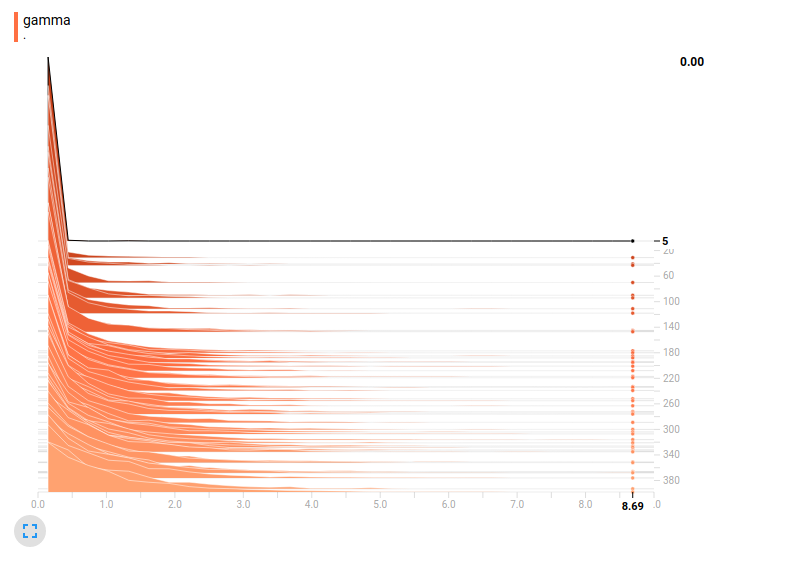
\includegraphics[scale=0.5]{tb_hist7.png}
\end{figure}
\end{center}
\begin{center}
\begin{figure}
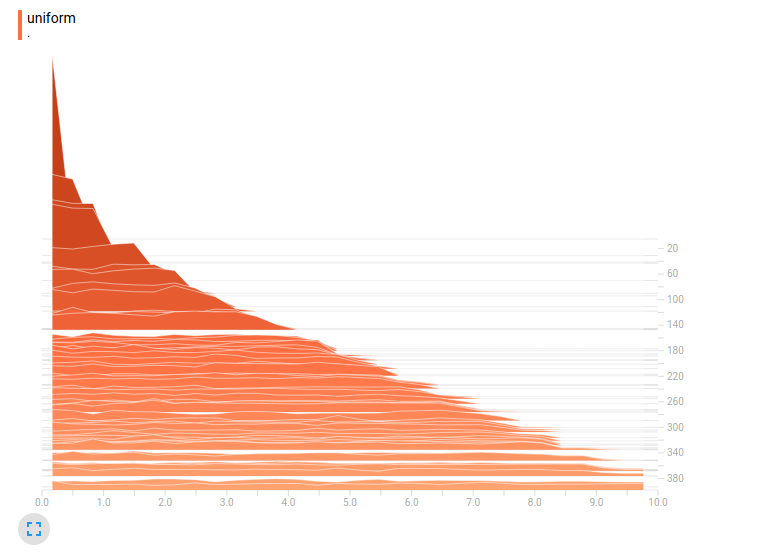
\includegraphics[scale=0.5]{tb_hist9.png}
\end{figure}
\end{center}
\subsection{poisson分布}
\begin{center}
\begin{figure}[H]
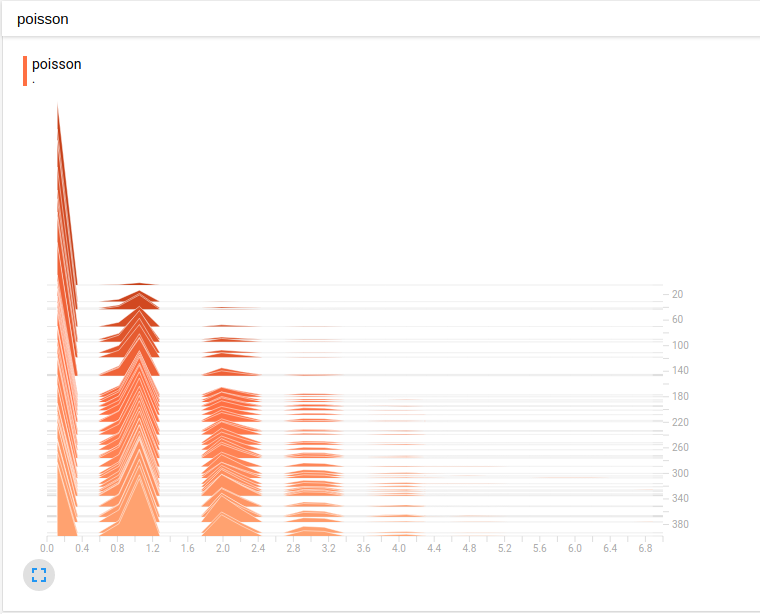
\includegraphics[scale=0.5]{tb_hist10.png}
\end{figure}
\end{center}
poisson分布定义在整数上,因此所有被生成的值都是整数,直方图压缩移动数据到浮点bins,导致可视化在整数值上显示一点点突起。
\subsection{结合所有的数据到一张图向上}
\begin{center}
\begin{figure}[H]
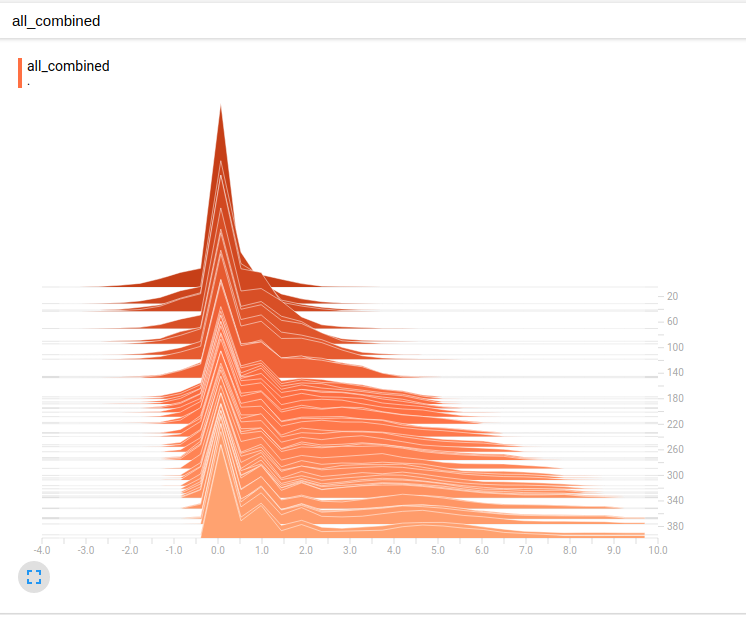
\includegraphics[scale=0.5]{tb_hist11.png}
\end{figure}
\end{center}


\begin{python}
import tensorflow as tf
import matplotlib.pyplot as plt
import numpy as np
tf.set_random_seed(0)
np.random.seed(0)
x = np.linspace(-1,1,100).reshape(-1,1)
noise = np.random.normal(0,0.1,size=x.shape)
y = np.power(x,2)+noise
def gendata():
    t = np.linspace(-1,1,100).reshape(-1,1)
def save():
    print('This is save')
    tf_x = tf.placeholder(tf.float32,x.shape)
    tf_y = tf.placeholder(tf.float32,y.shape)
    l = tf.layers.dense(tf_x,10,tf.nn.relu)
    o = tf.layers.dense(l,1)
    loss = tf.losses.mean_squared_error(tf_y,o)
    train_op = tf.train.GradientDescentOptimizer(learning_rate=0.5).minimize(loss)
    sess = tf.Session()
    sess.run(tf.global_variables_initializer())
    saver = tf.train.Saver()
    for step in range(100):
        sess.run(train_op,{tf_x:x,tf_y:y})
    saver.save(sess,'params',write_meta_graph=False)
    pred,l = sess.run([o,loss],{tf_x:x,tf_y:y})
    plt.figure(1,figsize=(10,5))
    plt.subplot(121)
    plt.scatter(x,y)
    plt.plot(x,pred,'r-',lw=5)
    plt.text(-1,1.2,'save loss=%.4f'%l,fontdict={'size':15,'color':'red'})
def reload():
    print('This is reload')
    tf_x = tf.placeholder(tf.float32,x.shape)
    tf_y = tf.placeholder(tf.float32,y.shape)
    l_ = tf.layers.dense(tf_x,10,tf.nn.relu)
    o_ = tf.layers.dense(l_,1)
    loss_ = tf.losses.mean_squared_error(tf_y,o_)
    sess = tf.Session()
    saver = tf.train.Saver()
    saver.restore(sess,'params')
    pred,l = sess.run([o_,loss_],{tf_x:x,tf_y:y})
    plt.subplot(122)
    plt.scatter(x,y)
    plt.plot(x,pred,'r-',lw=5)
    plt.text(-1,1.2,'Reload Loss=%.4f'%l,fontdict={'size':15,'color':'red'})
    plt.show()
save()
tf.reset_default_graph()
reload()
\end{python}
\section{CNN手写体数据识别}
\subsection{mnist数据集}
手写体数据训练集有55000张手写体数据图片。测试集有10000张图片。每张图片是大小为32*32的灰度图片。
卷积神经网络结构:
\begin{itemize}
	\item 第一层卷积层:卷积核16个,卷积核大小为$5\times5$,strides=1,padding为SAME,激活函数为relu(输出大小为$28\times28\times16$)。
	\item 第一层池化层:池化层大小为2,strides为2($14\times14\times16$)。
第二层卷积层:卷积核32,大小为$5\times5$,strides=1,padding为SAME,激活函数为relu。($14\times14\times32$)
	\item 第二层池化层:池化层大小为2,strides为2($7\times7\times32$)。
	\item flatten:1568。
\end{itemize}
\begin{figure}[H]
	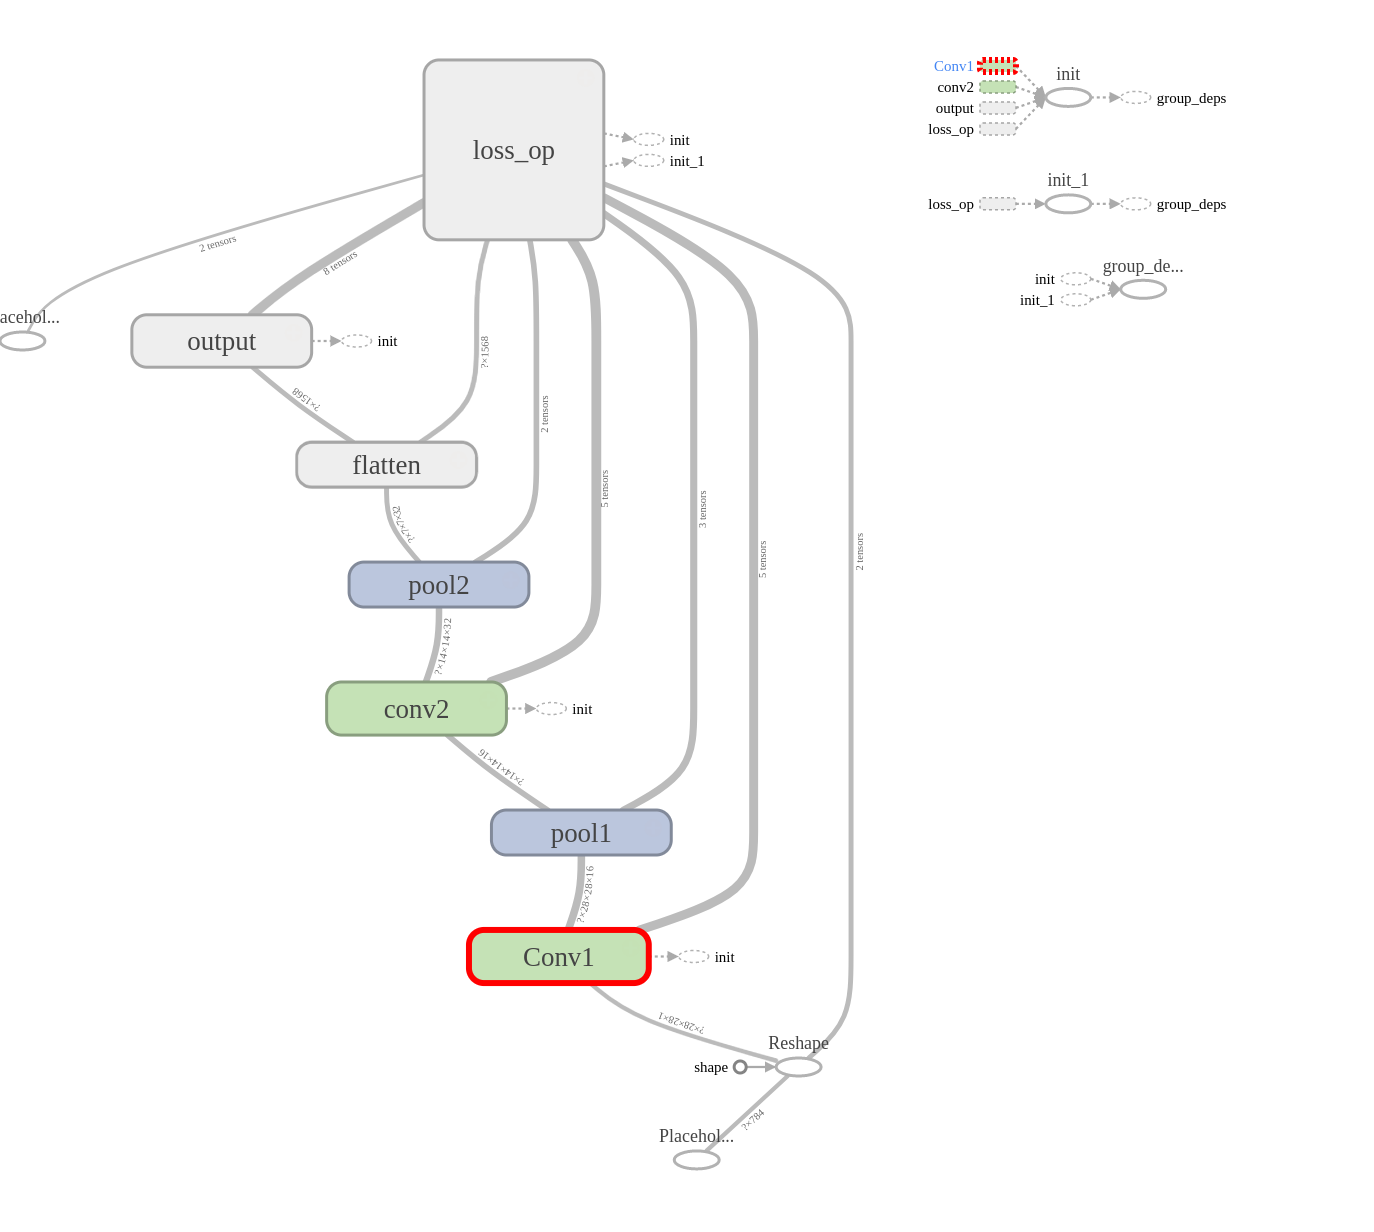
\includegraphics[scale=0.4]{./pic/chapter1/mnist_cnn.png}
\end{figure}
\begin{python}
import tensorflow as tf
import matplotlib.pyplot as plt
import numpy as np
from tensorflow.examples.tutorials.mnist import input_data

tf.set_random_seed(0)
np.random.seed(0)

BATCH_SIZE = 50
LR = 0.001
mnist = input_data.read_data_sets('/home/hpc/文档/mnist_tutorial/mnist',one_hot = True)
test_x = mnist.test.images[:2000]
test_y = mnist.test.labels[:2000]

tf_x = tf.placeholder(tf.float32,[None,28*28])
images = tf.reshape(tf_x,[-1,28,28,1])
tf_y = tf.placeholder(tf.int32,[None,10])
with tf.variable_scope('Conv1'):
    conv1 = tf.layers.conv2d(
            inputs = images,
            filters = 16,
            kernel_size = 5,
            strides = 1,
            padding = 'same',
            activation = tf.nn.relu
        )
    tf.summary.histogram('conv1',conv1)
with tf.variable_scope('pool1'):
    pool1 = tf.layers.max_pooling2d(
            conv1,
            pool_size=2,
            strides =2
        )
    tf.summary.histogram('max_pool1',pool1)
with tf.variable_scope('conv2'):
    conv2 = tf.layers.conv2d(pool1,32,5,1,'SAME',activation=tf.nn.relu)
    tf.summary.histogram('conv2',conv2)
with tf.variable_scope('pool2'):
    pool2 = tf.layers.max_pooling2d(conv2,2,2)
    tf.summary.histogram('max_pool',pool2)
with tf.variable_scope('flatten'):
    flat = tf.reshape(pool2,[-1,7*7*32])
with tf.variable_scope('output'):
    output = tf.layers.dense(flat,10)
with tf.variable_scope('loss_op'):
    loss = tf.losses.softmax_cross_entropy(onehot_labels=tf_y,logits=output)
    train_op = tf.train.AdamOptimizer(LR).minimize(loss)
    accuracy = tf.metrics.accuracy(labels = tf.argmax(tf_y,axis=1),predictions=tf.argmax(output,axis=1),)[1]
    tf.summary.scalar('loss',loss)
    tf.summary.scalar('accuracy',accuracy)
sess = tf.Session()
merge_op = tf.summary.merge_all()
init_op = tf.group(tf.global_variables_initializer(),tf.local_variables_initializer())
sess.run(init_op)
writer = tf.summary.FileWriter('./log',sess.graph)
for step in range(600):
    b_x,b_y = mnist.train.next_batch(BATCH_SIZE)
    _,loss_,result = sess.run([train_op,loss,merge_op],{tf_x:b_x,tf_y:b_y})
    writer.add_summary(result,step)
    if step%50 == 0:
        accuracy_,flat_representation = sess.run([accuracy,flat],{tf_x:test_x,tf_y:test_y})
        print('Step:',step,'| train loss:%.4f'%loss_,'|test accuracy:%.2f'%accuracy_)
test_output = sess.run(output,{tf_x:test_x[:10]})
pred_y = np.argmax(test_output,1)
\end{python}
\section{RNN}
\subsection{向量字表示}
\subsubsection{Vector Representation of Words}
通常图像或音频系统处理的是由图片中所有单个原始像素点强度值或者音频中功率谱密度的强度值,把它们编码成丰富、高维度的向量数据集。对于物体或语音识别这一类的任务,我们所需的全部信息已经都存储在原始数据中(显然人类本身就是依赖原始数据进行日常的物体或语音识别的)。然后,自然语言处理系统通常将词汇作为离散的单一符号,例如 "cat" 一词或可表示为 Id537 ,而 "dog" 一词或可表示为 Id143。这些符号编码毫无规律,无法提供不同词汇之间可能存在的关联信息。换句话说,在处理关于 "dogs" 一词的信息时,模型将无法利用已知的关于 "cats" 的信息(例如,它们都是动物,有四条腿,可作为宠物等等)。可见,将词汇表达为上述的独立离散符号将进一步导致数据稀疏,使我们在训练统计模型时不得不寻求更多的数据。而词汇的向量表示将克服上述的难题。向量空间模型 (VSMs)将词汇表达(嵌套)于一个连续的向量空间中,语义近似的词汇被映射为相邻的数据点。向量空间模型在自然语言处理领域中有着漫长且丰富的历史,不过几乎所有利用这一模型的方法都依赖于 分布式假设,其核心思想为出现于上下文情景中的词汇都有相类似的语义。采用这一假设的研究方法大致分为以下两类:基于计数的方法 (e.g. 潜在语义分析), 和 预测方法 (e.g. 神经概率化语言模型).

其中它们的区别在如下论文中又详细阐述 \href{http://clic.cimec.unitn.it/marco/publications/acl2014/baroni-etal-countpredict-acl2014.pdf}{Baroni :et al},不过简而言之:基于计数的方法计算某词汇与其邻近词汇在一个大型语料库中共同出现的频率及其它统计量,然后将这些统计量映射到一个小型且稠密的向量中。预测方法则试图直接从某词汇的邻近词汇对其进行预测,在此过程中利用已经学习到的小型且稠密的嵌套向量。

Word2vec是一种可以进行高效率词嵌套学习的预测模型。其两种变体分别为:连续词袋模型(CBOW)及Skip-Gram模型。从算法角度看,这两种方法非常相似,其区别为CBOW根据源词上下文词汇('the cat sits on the')来预测目标词汇(例如,‘mat’),而Skip-Gram模型做法相反,它通过目标词汇来预测源词汇。Skip-Gram模型采取CBOW的逆过程的动机在于:CBOW算法对于很多分布式信息进行了平滑处理(例如将一整段上下文信息视为一个单一观察量)。很多情况下,对于小型的数据集,这一处理是有帮助的。相形之下,Skip-Gram模型将每个“上下文-目标词汇”的组合视为一个新观察量,这种做法在大型数据集中会更为有效。本教程余下部分将着重讲解Skip-Gram模型。
\subsubsection{处理噪声的对比训练}
神经概率化语言模型通常使用极大似然法 (ML) 进行训练,其中通过 softmax function 来最大化当提供前一个单词 h (代表 "history"),后一个单词的概率$w_t$(目标词概率)
\begin{equation*}
P(w_t|h)=softmax(score(w_t,h))=\frac{exp\left\{score(w_t,h)\right\}}{\Sigma_{Word w' in Vocab}exp\left\{score(w',h)\right\}}
\end{equation*}
当 $score(w_t,h)$ 计算了文字 $w_t$ 和 上下文 h 的相容性(通常使用向量积)。我们使用对数似然函数来训练训练集的最大值,比如通过:
\begin{equation*}
J_{ML} = logP(w_t|h)=score(w_t,h)-log(\Sigma_{Word w' in Vocab}exp\left\{score(w',h)\right\})
\end{equation*}
这里提出了一个解决语言概率模型的合适的通用方法。然而这个方法实际执行起来开销非常大,因为我们需要去计算并正则化当前上下文环境 h 中所有其它 V 单词 w' 的概率得分,在每一步训练迭代中。
\begin{figure}[H]
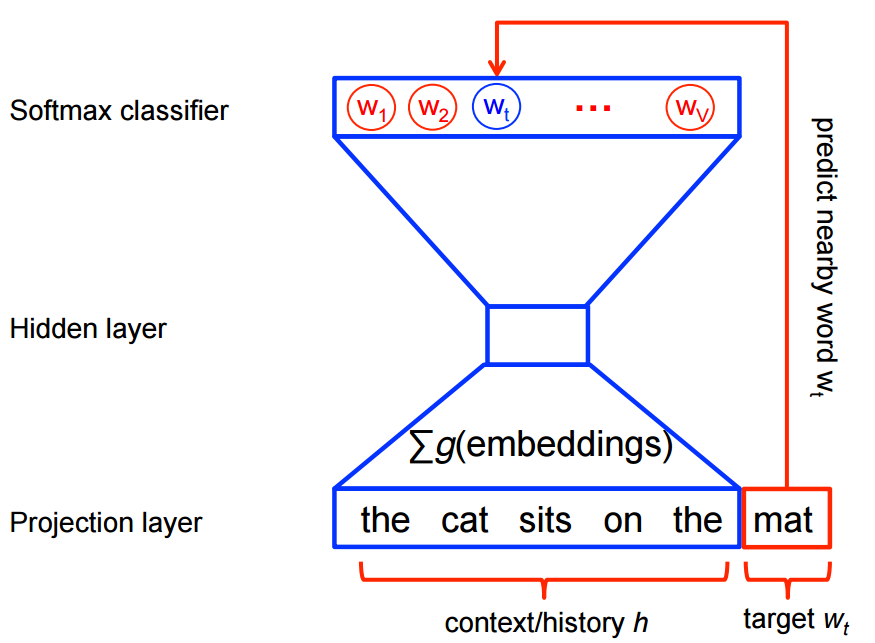
\includegraphics[scale=0.5]{softmax-nplm.png}
\caption{CBOW方法}
\end{figure}
从另一个角度来说,当使用word2vec模型时,我们并不需要对概率模型中的所有特征进行学习。而CBOW模型和Skip-Gram模型为了避免这种情况发生,使用一个二分类器(逻辑回归)在同一个上下文环境里从 k 虚构的 (噪声) 单词$\hat{w}$区分真正的目标单词$w_t$,下面详细参数CBOW模型,对于Skip-Gram模型只要简单的反向操作即可。
\begin{center}
\begin{figure}[H]
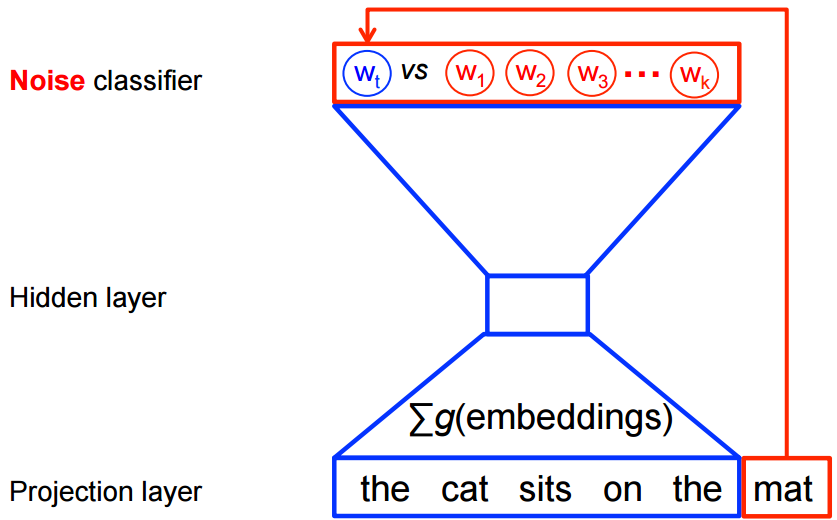
\includegraphics[scale=0.5]{nce-nplm.png}
\caption{Skip-Gram}
\end{figure}
\end{center}
从数学的角度来说,我们的目标是对每个样本最大化:
\begin{equation*}
J_{NEG}=logQ_{\theta}(D=1|w_t,h)+k\underset{\hat{w}\sim P_{noise}}{E}[logQ_{\theta}(D=0|\hat{\omega},h)]
\end{equation*}
其中$Q_{\theta}(D=1|w,h)$代表的是当前上下文h,根据所学得嵌套向量$\theta$目标单词 w 使用二分类逻辑回归计算得出的概率。在实践中,我们通过在噪声分布中绘制比对文字来获得近似的期望值(通过计算\href{https://en.wikipedia.org/wiki/Monte_Carlo_integration}{蒙特卡洛平均值})。

当真实地目标单词被分配到较高的概率,同时噪声单词的概率很低时,目标函数也就达到最大值了。从技术层面来说,这种方法叫做\href{http://papers.nips.cc/paper/5021-distributed-representations-of-words-and-phrases-and-their-compositionality.pdf}{负抽样},而且使用这个损失函数在数学层面上也有很好的解释:这个更新过程也近似于softmax函数的更新。这在计算上将会有很大的优势,因为当计算这个损失函数时,只是有我们挑选出来的 k 个 噪声单词,而没有使用整个语料库 V。这使得训练变得非常快。我们实际上使用了与\href{http://papers.nips.cc/paper/5165-learning-word-embeddings-efficiently-with-noise-contrastive-estimation.pdf}{noise-contrastive estimation (NCE)}介绍的非常相似的方法,这在TensorFlow中已经封装了一个很便捷的函数tf.nn.nce\_loss()。

\subsubsection{Skip-gram模型}
下面来看一下这个数据集

the quick brown fox jumped over the lazy dog

我们首先对一些单词以及它们的上下文环境建立一个数据集。我们可以以任何合理的方式定义‘上下文’,而通常上这个方式是根据文字的句法语境的(使用语法原理的方式处理当前目标单词可以看一下这篇文献 \href{https://levyomer.files.wordpress.com/2014/04/dependency-based-word-embeddings-acl-2014.pdf}{Levy et al.},比如说把目标单词左边的内容当做一个‘上下文’,或者以目标单词右边的内容,等等。现在我们把目标单词的左右单词视作一个上下文, 使用大小为1的窗口,这样就得到这样一个由(上下文, 目标单词) 组成的数据集:

([the, brown], quick), ([quick, fox], brown), ([brown, jumped], fox), ...

前文提到Skip-Gram模型是把目标单词和上下文颠倒过来,所以在这个问题中,举个例子,就是用'quick'来预测 'the' 和 'brown' ,用 'brown' 预测 'quick' 和 'brown' 。因此这个数据集就变成由(输入, 输出)组成的:

(quick, the), (quick, brown), (brown, quick), (brown, fox), ...

目标函数通常是对整个数据集建立的,但是本问题中要对每一个样本(或者是一个batch\_size 很小的样本集,通常设置为16 <= batch\_size <= 512)在同一时间执行特别的操作,称之为\href{https://en.wikipedia.org/wiki/Stochastic_gradient_descent}{随机梯度下降 (SGD)}。我们来看一下训练过程中每一步的执行。

假设用 t 表示上面这个例子中quick 来预测 the 的训练的单个循环。用 num\_noise 定义从噪声分布中挑选出来的噪声(相反的)单词的个数,通常使用一元分布,P(w)。为了简单起见,我们就定num\_noise=1,用 sheep 选作噪声词。接下来就可以计算每一对观察值和噪声值的损失函数了,每一个执行步骤就可表示为:
\begin{equation*}
J_{NEG}^{(t)}=logQ_{\theta}(D=1|the,quick)+log(Q_{\theta}(D=0|sleep,quick))
\end{equation*}
整个计算过程的目标是通过更新嵌套参数$\theta$来逼近目标函数(这个例子中就是使目标函数最大化)。为此我们要计算损失函数中嵌套参数$\theta$的梯度,比如\[\frac{\partial}{\partial}J_{NEG}\]
(幸好TensorFlow封装了工具函数可以简单调用!)。对于整个数据集,当梯度下降的过程中不断地更新参数,对应产生的效果就是不断地移动每个单词的嵌套向量,直到可以把真实单词和噪声单词很好得区分开。

我们可以把学习向量映射到2维中以便我们观察,其中用到的技术可以参考 \href{http://lvdmaaten.github.io/tsne/}{t-SNE 降维技术}。当我们用可视化的方式来观察这些向量,就可以很明显的获取单词之间语义信息的关系,这实际上是非常有用的。当我们第一次发现这样的诱导向量空间中,展示了一些特定的语义关系,这是非常有趣的,比如文字中 male-female,gender 甚至还有 country-capital 的关系, 如下方的图所示 (也可以参考 \href{http://www.aclweb.org/anthology/N13-1090}{Mikolov et al.}, 2013论文中的例子)。
\begin{center}
\begin{figure}[H]
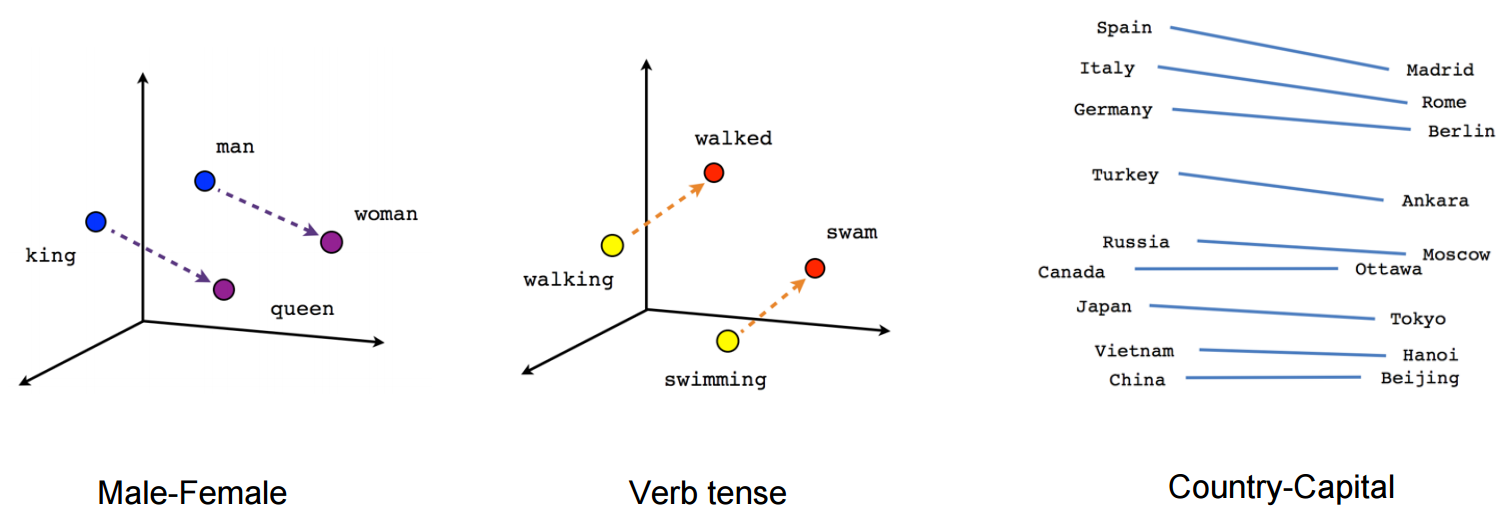
\includegraphics[scale=0.5]{linear-relationships.png}
\end{figure}
\end{center}
这也解释了为什么这些向量在传统的NLP问题中可作为特性使用,比如用在对一个演讲章节打个标签,或者对一个专有名词的识别 (看看如下这个例子 \href{https://arxiv.org/pdf/1103.0398v1.pdf}{Collobert et al.}或者 \href{http://www.aclweb.org/anthology/P10-1040}{Turian et al.})。

不过现在让我们用它们来画漂亮的图表吧!

这里谈得都是嵌套,那么先来定义一个嵌套参数矩阵。我们用唯一的随机值来初始化这个大矩阵。
\begin{python}
embeddings = tf.Variable(
    tf.random_uniform([vocabulary_size, embedding_size], -1.0, 1.0))
\end{python}
对噪声-比对的损失计算就使用一个逻辑回归模型。对此,我们需要对语料库中的每个单词定义一个权重值和偏差值。(也可称之为输出权重 与之对应的 输入嵌套值)。定义如下:
\begin{python}
nce_weights = tf.Variable(
  tf.truncated_normal([vocabulary_size, embedding_size],
                      stddev=1.0 / math.sqrt(embedding_size)))
nce_biases = tf.Variable(tf.zeros([vocabulary_size]))
\end{python}我们有了这些参数之后,就可以定义Skip-Gram模型了。简单起见,假设我们已经把语料库中的文字整型化了,这样每个整型代表一个单词(细节请查看\_basic.py)。Skip-Gram模型有两个输入。一个是一组用整型表示的上下文单词,另一个是目标单词。给这些输入建立占位符节点,之后就可以填入数据了。
\begin{python}
train_inputs = tf.placeholder(tf.int32, shape=[batch_size])
train_labels = tf.placeholder(tf.int32, shape=[batch_size, 1])
\end{python}
然后我们需要对批数据中的单词建立嵌套向量,TensorFlow提供了方便的工具函数。
\begin{python}
embed = tf.nn.embedding_lookup(embeddings, train_inputs)
\end{python}
好了,现在我们有了每个单词的嵌套向量,接下来就是使用噪声-比对的训练方式来预测目标单词。
\begin{python}
loss = tf.reduce_mean(
  tf.nn.nce_loss(nce_weights, nce_biases, embed, train_labels,
                 num_sampled, vocabulary_size))
\end{python}
我们对损失函数建立了图形节点,然后我们需要计算相应梯度和更新参数的节点,比如说在这里我们会使用随机梯度下降法,TensorFlow也已经封装好了该过程。
\begin{python}
optimizer = tf.train.GradientDescentOptimizer(learning_rate=1.0).minimize(loss)
\end{python}
\subsubsection{训练过程}
训练的过程很简单,只要在循环中使用feed\_dict不断给占位符填充数据,同时调用 session.run即可。
\begin{python}
for inputs, labels in generate_batch(...):
  feed_dict = {training_inputs: inputs, training_labels: labels}
  _, cur_loss = session.run([optimizer, loss], feed_dict=feed_dict)
\end{python}
\subsubsection{嵌套学习结果可视化}
\begin{center}
\begin{figure}[H]
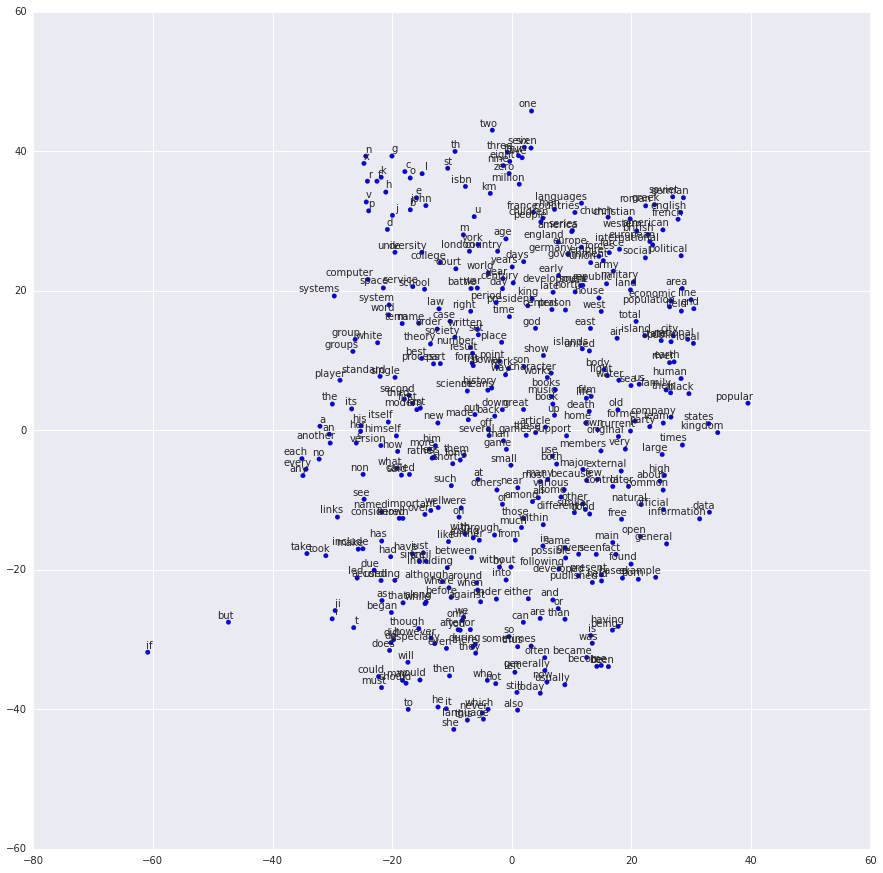
\includegraphics[scale=0.5]{tsne.png}
\end{figure}
\end{center}
Et voila! 与预期的一样,相似的单词被聚类在一起。对word2vec模型更复杂的实现需要用到TensorFlow一些更高级的特性,具体是实现可以参考\href{https://github.com/bleedingfight/models/tree/master/tutorials/embedding}{word2vec.py}\subsubsection{嵌套学习的评估:类比推理}
词嵌套在NLP的预测问题中是非常有用且使用广泛地。如果要检测一个模型是否是可以成熟地区分词性或者区分专有名词的模型,最简单的办法就是直接检验它的预测词性、语义关系的能力,比如让它解决形如king is to queen as father is to ?这样的问题。这种方法叫做类比推理 ,可参考Mikolov and colleagues,数据集下载地址为:\href{https://word2vec.googlecode.com/svn/trunk/questions-words.txt}{questions-words.txt} 。
To see how we do this evaluation如何执行这样的评估,可以看build\_eval\_graph()和 eval()这两个函数在下面源码中的使用 \href{https://github.com/bleedingfight/models/tree/master/tutorials/embedding}{word2vec.py}

超参数的选择对该问题解决的准确性有巨大的影响。想要模型具有很好的表现,需要有一个巨大的训练数据集,同时仔细调整参数的选择并且使用例如二次抽样的一些技巧。不过这些问题已经超出了本教程的范围。
\subsubsection{优化实现}
以上简单的例子展示了TensorFlow的灵活性。比如说,我们可以很轻松得用现成的tf.nn.sampled\_softmax\_loss()来代替tf.nn.nce\_loss()构成目标函数。如果你对损失函数想做新的尝试,你可以用TensorFlow手动编写新的目标函数的表达式,然后用控制器执行计算。这种灵活性的价值体现在,当我们探索一个机器学习模型时,我们可以很快地遍历这些尝试,从中选出最优。

一旦你有了一个满意的模型结构,或许它就可以使实现运行地更高效(在短时间内覆盖更多的数据)。比如说,在本教程中使用的简单代码,实际运行速度都不错,因为我们使用Python来读取和填装数据,而这些在TensorFlow后台只需执行非常少的工作。如果你发现你的模型在输入数据时存在严重的瓶颈,你可以根据自己的实际问题自行实现一个数据阅读器,参考 新的数据格式。对于Skip-Gram 模型,我们已经完成了如下这个例子 \href{https://github.com/bleedingfight/models/tree/master/tutorials/embedding}{word2vec.py}。

如果I/O问题对你的模型已经不再是个问题,并且想进一步地优化性能,或许你可以自行编写TensorFlow操作单元,详见 添加一个新的操作。相应的,我们也提供了Skip-Gram模型的例子 \href{https://github.com/bleedingfight/models/tree/master/tutorials/embedding}{optimized.py}。请自行调节以上几个过程的标准,使模型在每个运行阶段有更好地性能。
\subsection{RNN}
此教程将展示如何在高难度的语言模型中训练循环神经网络。该问题的目标是获得一个能确定语句概率的概率模型。为了做到这一点,通过之前已经给出的词语来预测后面的词语。我们将使用 PTB(Penn Tree Bank) 数据集,这是一种常用来衡量模型的基准,同时它比较小而且训练起来相对快速。

语言模型是很多有趣难题的关键所在,比如语音识别,机器翻译,图像字幕等。它很有意思--可以参看 here。

本教程的目的是重现 \href{http://arxiv.org/abs/1409.2329}{Zaremba et al., 2014} 的成果,他们在 PTB 数据集上得到了很棒的结果。
\subsubsection{下载及准备数据}
本教程需要的数据在 data/ 路径下,来源于 Tomas Mikolov 网站上的\href{http://www.fit.vutbr.cz/~imikolov/rnnlm/simple-examples.tg}{PTB 数据集}

该数据集已经预先处理过并且包含了全部的 10000 个不同的词语,其中包括语句结束标记符,以及标记稀有词语的特殊符号 (<unk>) 。我们在 reader.py 中转换所有的词语,让他们各自有唯一的整型标识符,便于神经网络处理。
\subsubsection{LSTM}
模型的核心由一个 LSTM 单元组成,其可以在某时刻处理一个词语,以及计算语句可能的延续性的概率。网络的存储状态由一个零矢量初始化并在读取每一个词语后更新。而且,由于计算上的原因,我们将以 batch\_size 为最小批量来处理数据。

基础的伪代码就像下面这样:
\begin{python}
lstm = rnn_cell.BasicLSTMCell(lstm_size)
state = tf.zeros([batch_size, lstm.state_size])

loss = 0.0
for current_batch_of_words in words_in_dataset:
    output, state = lstm(current_batch_of_words, state)

    logits = tf.matmul(output, softmax_w) + softmax_b
    probabilities = tf.nn.softmax(logits)
    loss += loss_function(probabilities, target_words)
\end{python}
\subsubsection{截断反向传播}
为使学习过程易于处理,通常的做法是将反向传播的梯度在(按时间)展开的步骤上照一个固定长度(num\_steps)截断。 通过在一次迭代中的每个时刻上提供长度为 num\_steps 的输入和每次迭代完成之后反向传导,这会很容易实现。

一个简化版的用于计算图创建的截断反向传播代码:
\begin{python}
words = tf.placeholder(tf.int32, [batch_size, num_steps])

lstm = rnn_cell.BasicLSTMCell(lstm_size)
initial_state = state = tf.zeros([batch_size, lstm.state_size])

for i in range(len(num_steps)):
    output, state = lstm(words[:, i], state)

    # ...

final_state = state
\end{python}
下面展现如何实现迭代整个数据集:
\begin{python}
numpy_state = initial_state.eval()
total_loss = 0.0
for current_batch_of_words in words_in_dataset:
    numpy_state, current_loss = session.run([final_state, loss],
        feed_dict={initial_state: numpy_state, words: current_batch_of_words})
    total_loss += current_loss
\end{python}
\subsubsection{输入}
在输入 LSTM 前,词语 ID 被嵌入到了一个密集的表示中(查看 矢量表示教程)。这种方式允许模型高效地表示词语,也便于写代码:
\begin{python}
# embedding_matrix 张量的形状是: [vocabulary_size, embedding_size]
word_embeddings = tf.nn.embedding_lookup(embedding_matrix, word_ids)
\end{python}
嵌入的矩阵会被随机地初始化,模型会学会通过数据分辨不同词语的意思。
\subsubsection{损失函数}
我们想使目标词语的平均负对数概率最小$loss = -\frac{1}{N}\Sigma_{i=1}^NlnP_{target_i}$
实现起来并非很难,而且函数 sequence\_loss\_by\_example 已经有了,可以直接使用。

论文中的典型衡量标准是每个词语的平均困惑度(perplexity),计算式为
$$e^{-\frac{1}{N}\Sigma_{i=1}^N}lnp_{target_i}=e^{loss}$$
同时我们会观察训练过程中的困惑度值(perplexity)
\subsubsection{多个LSTM层堆叠}
要想给模型更强的表达能力,可以添加多层 LSTM 来处理数据。第一层的输出作为第二层的输入,以此类推。

类 MultiRNNCell 可以无缝的将其实现:
\begin{python}
lstm = rnn_cell.BasicLSTMCell(lstm_size)
stacked_lstm = rnn_cell.MultiRNNCell([lstm] * number_of_layers)

initial_state = state = stacked_lstm.zero_state(batch_size, tf.float32)
for i in range(len(num_steps)):
    # 每次处理一批词语后更新状态值.
    output, state = stacked_lstm(words[:, i], state)

    # 其余的代码.
    # ...

final_state = state
\end{python}
\subsubsection{编译并运行代码}
首先需要构建库,在CPU上编译:
\begin{python}
bazel build -c opt tensorflow/models/rnn/ptb:ptb_word_lm
\end{python}
如果你有一个强大的 GPU,可以运行
\begin{python}
bazel build -c opt --config=cuda tensorflow/models/rnn/ptb:ptb_word_lm
\end{python}
运行模型:
\begin{python}
bazel-bin/tensorflow/models/rnn/ptb/ptb_word_lm \
  --data_path=/tmp/simple-examples/data/ --alsologtostderr --model small
\end{python}
教程代码中有 3 个支持的模型配置参数:"small", "medium" 和 "large"。它们指的是 LSTM 的大小,以及用于训练的超参数集。

模型越大,得到的结果应该更好。在测试集中 small 模型应该可以达到低于 120 的困惑度(perplexity),large 模型则是低于 80,但它可能花费数小时来训练。
